\documentclass[twocolumn]{aastex631}

\usepackage{amsmath}
\usepackage{multirow}
\usepackage{natbib}
\usepackage{graphicx} 
\usepackage{aas_macros}

\begin{document}

\subsection{Data Preprocessing and Feature Engineering}

The initial dataset consisted of 1000 merger trees, originating from 40 unique N-body simulations, with 25 trees per simulation. Prior to feature engineering, node features, specifically the base-10 logarithm of halo mass (log10(mass)), the base-10 logarithm of halo concentration (log10(concentration)), the base-10 logarithm of the maximum circular velocity (log10(Vmax)), and the cosmological scale factor, were normalized. This normalization was performed using the mean and standard deviation computed solely from the training set (800 trees from 32 simulations). The computed normalization parameters, detailed in the file `data/normalization\_params.npz`, were: mean = `[11.138, 0.736, 2.115, 0.370]` and std = `[0.713, 0.364, 0.212, 0.180]` for the four node features, respectively.

A total of 24 engineered features were constructed for each graph, divided into three categories:
\begin{enumerate}
    \item Edge-based features (4): These features captured information about the merger events. They included the mean and variance of the absolute difference in scale factors between connected nodes, and the mean and variance of the log-ratio of descendant mass to progenitor mass.
    \item Laplacian spectral features (5): These features aimed to capture the global connectivity and structure of the merger trees. They included the mean, standard deviation, skewness, and kurtosis of the normalized graph Laplacian eigenvalues, as well as the sum of the 10 smallest non-zero eigenvalues.
    \item Diffusion map features (15): These features were derived from node embeddings obtained using diffusion maps. The top 5 eigenvectors of the random walk transition matrix were used to embed the nodes, and these embeddings were then aggregated at the graph level using mean, maximum, and minimum pooling (5 eigenvectors x 3 aggregation methods).
\end{enumerate}

A significant challenge was the computational cost associated with eigenvalue decomposition for large graphs. To address this, a threshold (`MAX\_NODES\_FOR\_EIGS = 500`) was set, above which Laplacian and diffusion feature calculations were skipped. This resulted in NaN values for these features in graphs exceeding this size limit. Specifically, 638 out of 800 training graphs and 164 out of 200 test graphs exceeded this limit. Consequently, a substantial number of NaN entries were present in the engineered feature matrices (12,760 NaNs in `X\_train\_engineered` (an 800x24 matrix) and 3,280 NaNs in `X\_test\_engineered` (a 200x24 matrix)), primarily affecting the 20 spectral and diffusion features. These NaNs were subsequently handled by mean imputation prior to Principal Component Analysis (PCA).

The distributions of the engineered features (post-imputation for plotting purposes where applicable, using raw values from `data/engineered\_features\_train.npz`) were visualized in a series of histograms. The distributions of the edge features (e.g., `mean\ensuremath{\_}delta\ensuremath{\_}sf` and `mean\ensuremath{\_}log\ensuremath{\_}mass\ensuremath{\_}ratio`) were relatively compact. However, the distributions of the Laplacian spectral features (e.g., `lap\ensuremath{\_}eig\ensuremath{\_}mean` and `lap\ensuremath{\_}eig\ensuremath{\_}std`) and the diffusion map features (mean, max, min pooled) were influenced by the imputation of NaNs for large graphs.

\begin{figure}[h!]
    \centering
    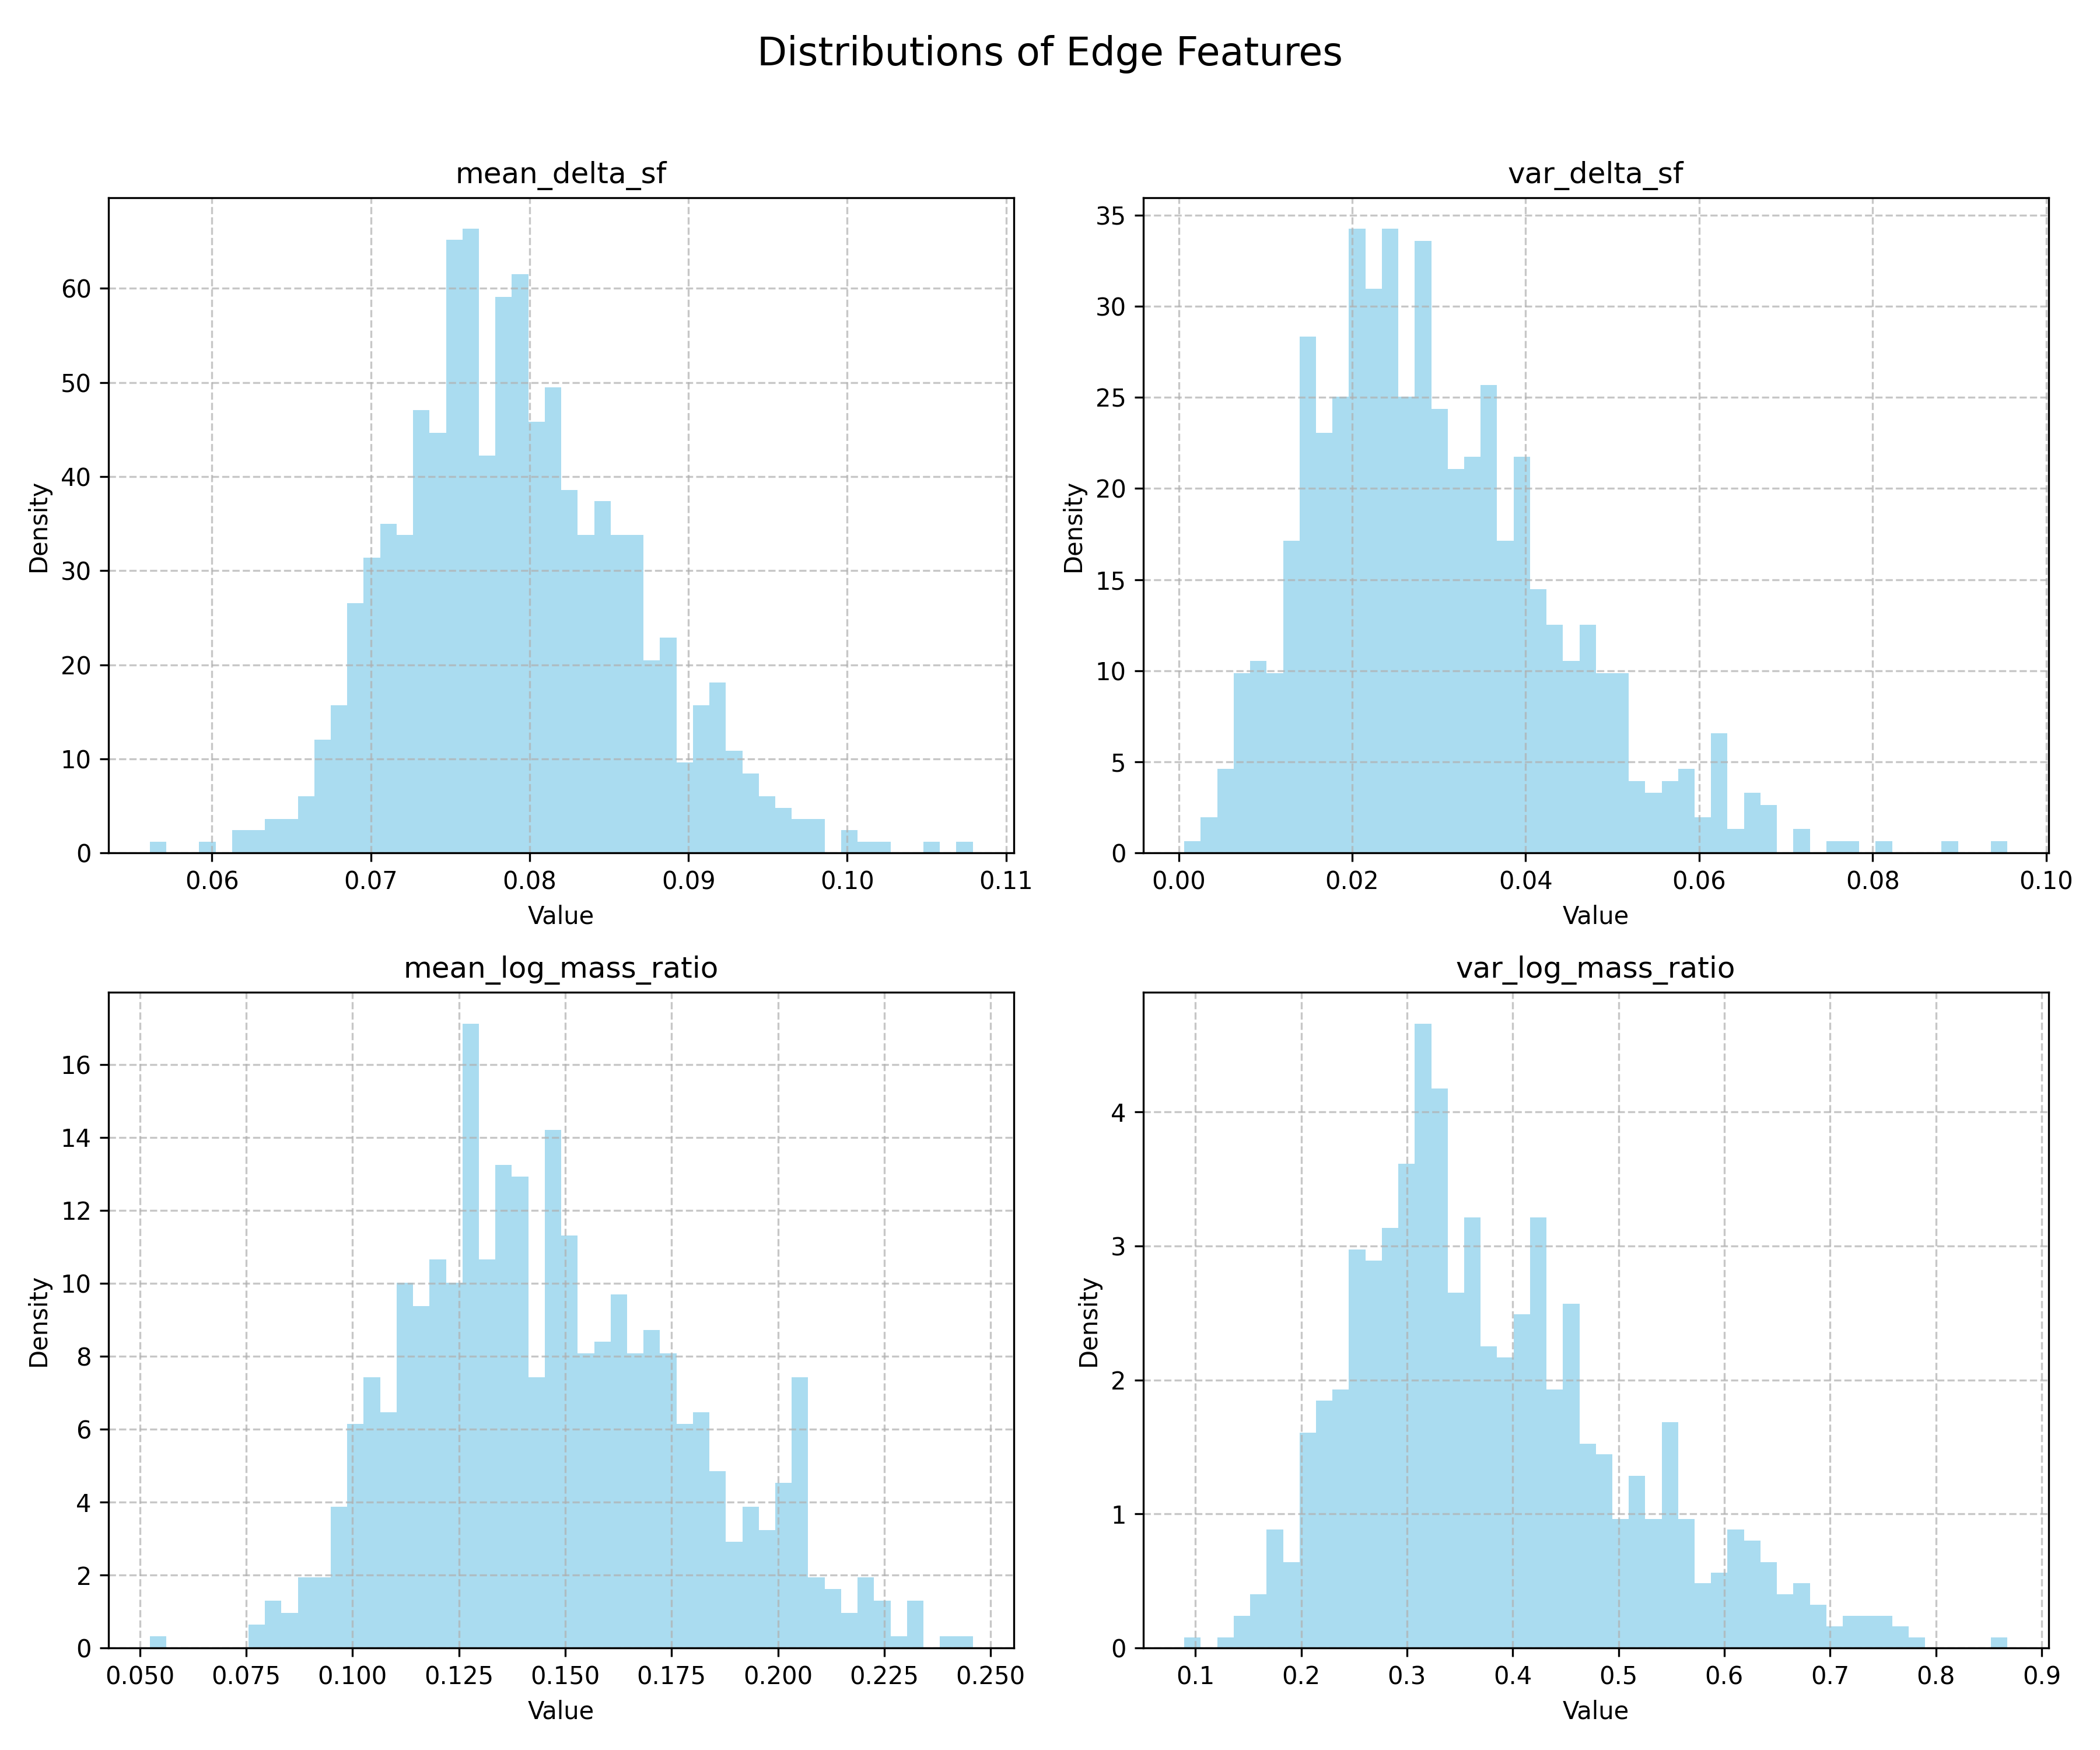
\includegraphics[width=0.5\textwidth]{../input_files/plots/engineered_feature_dist_edge_1_20250527-135752.png}
    \caption{Distributions of edge features (mean and variance of the absolute difference in scale factors between connected nodes, and mean and variance of the log-ratio of descendant mass to progenitor mass). These relatively compact distributions were used to predict cosmological parameters, but ultimately performed worse than simpler features.}
    \label{fig:edge_feature_dist}
\end{figure}

\begin{figure}[h!]
    \centering
    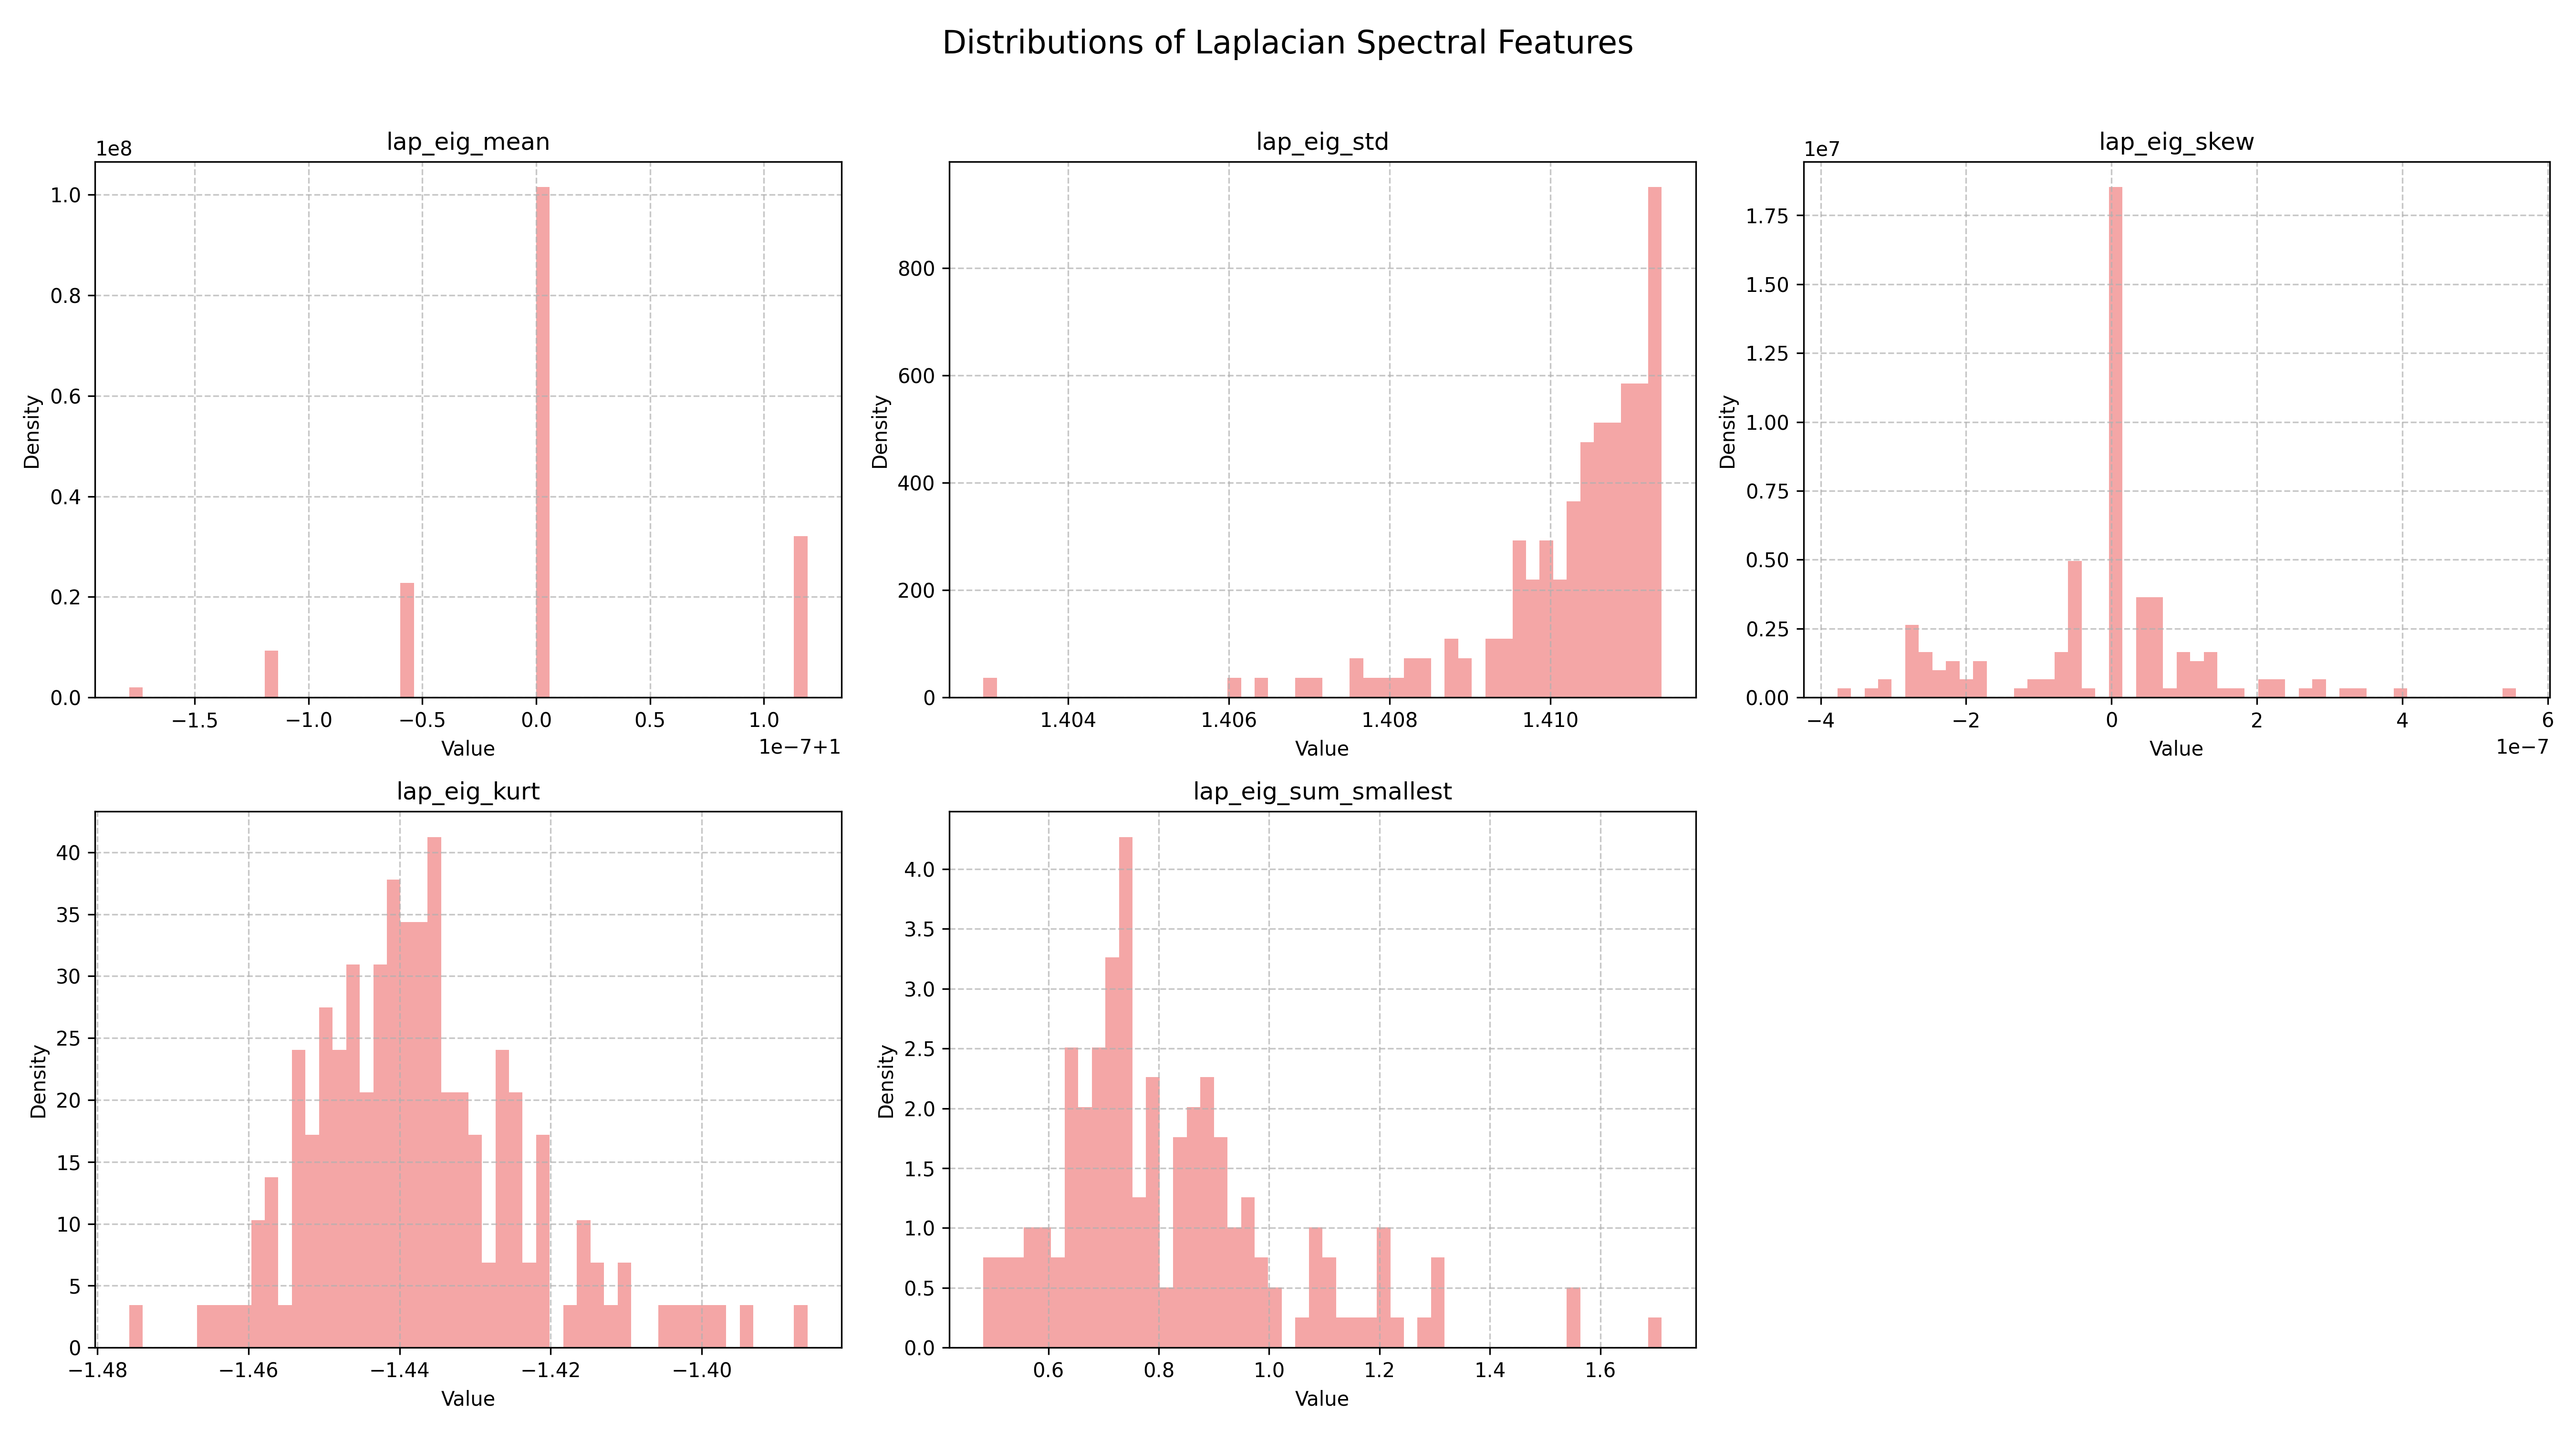
\includegraphics[width=0.5\textwidth]{../input_files/plots/engineered_feature_dist_laplacian_2_20250527-135752.png}
    \caption{Distributions of Laplacian spectral features (mean, standard deviation, skewness, kurtosis, and sum of the 10 smallest non-zero eigenvalues) across the training set merger trees. These features, intended to capture graph structure, were ultimately found to be poor predictors of cosmological parameters, likely due to the imputation of NaN values arising from computational limitations for large graphs.}
    \label{fig:laplacian_feature_dist}
\end{figure}

\begin{figure}[h!]
    \centering
    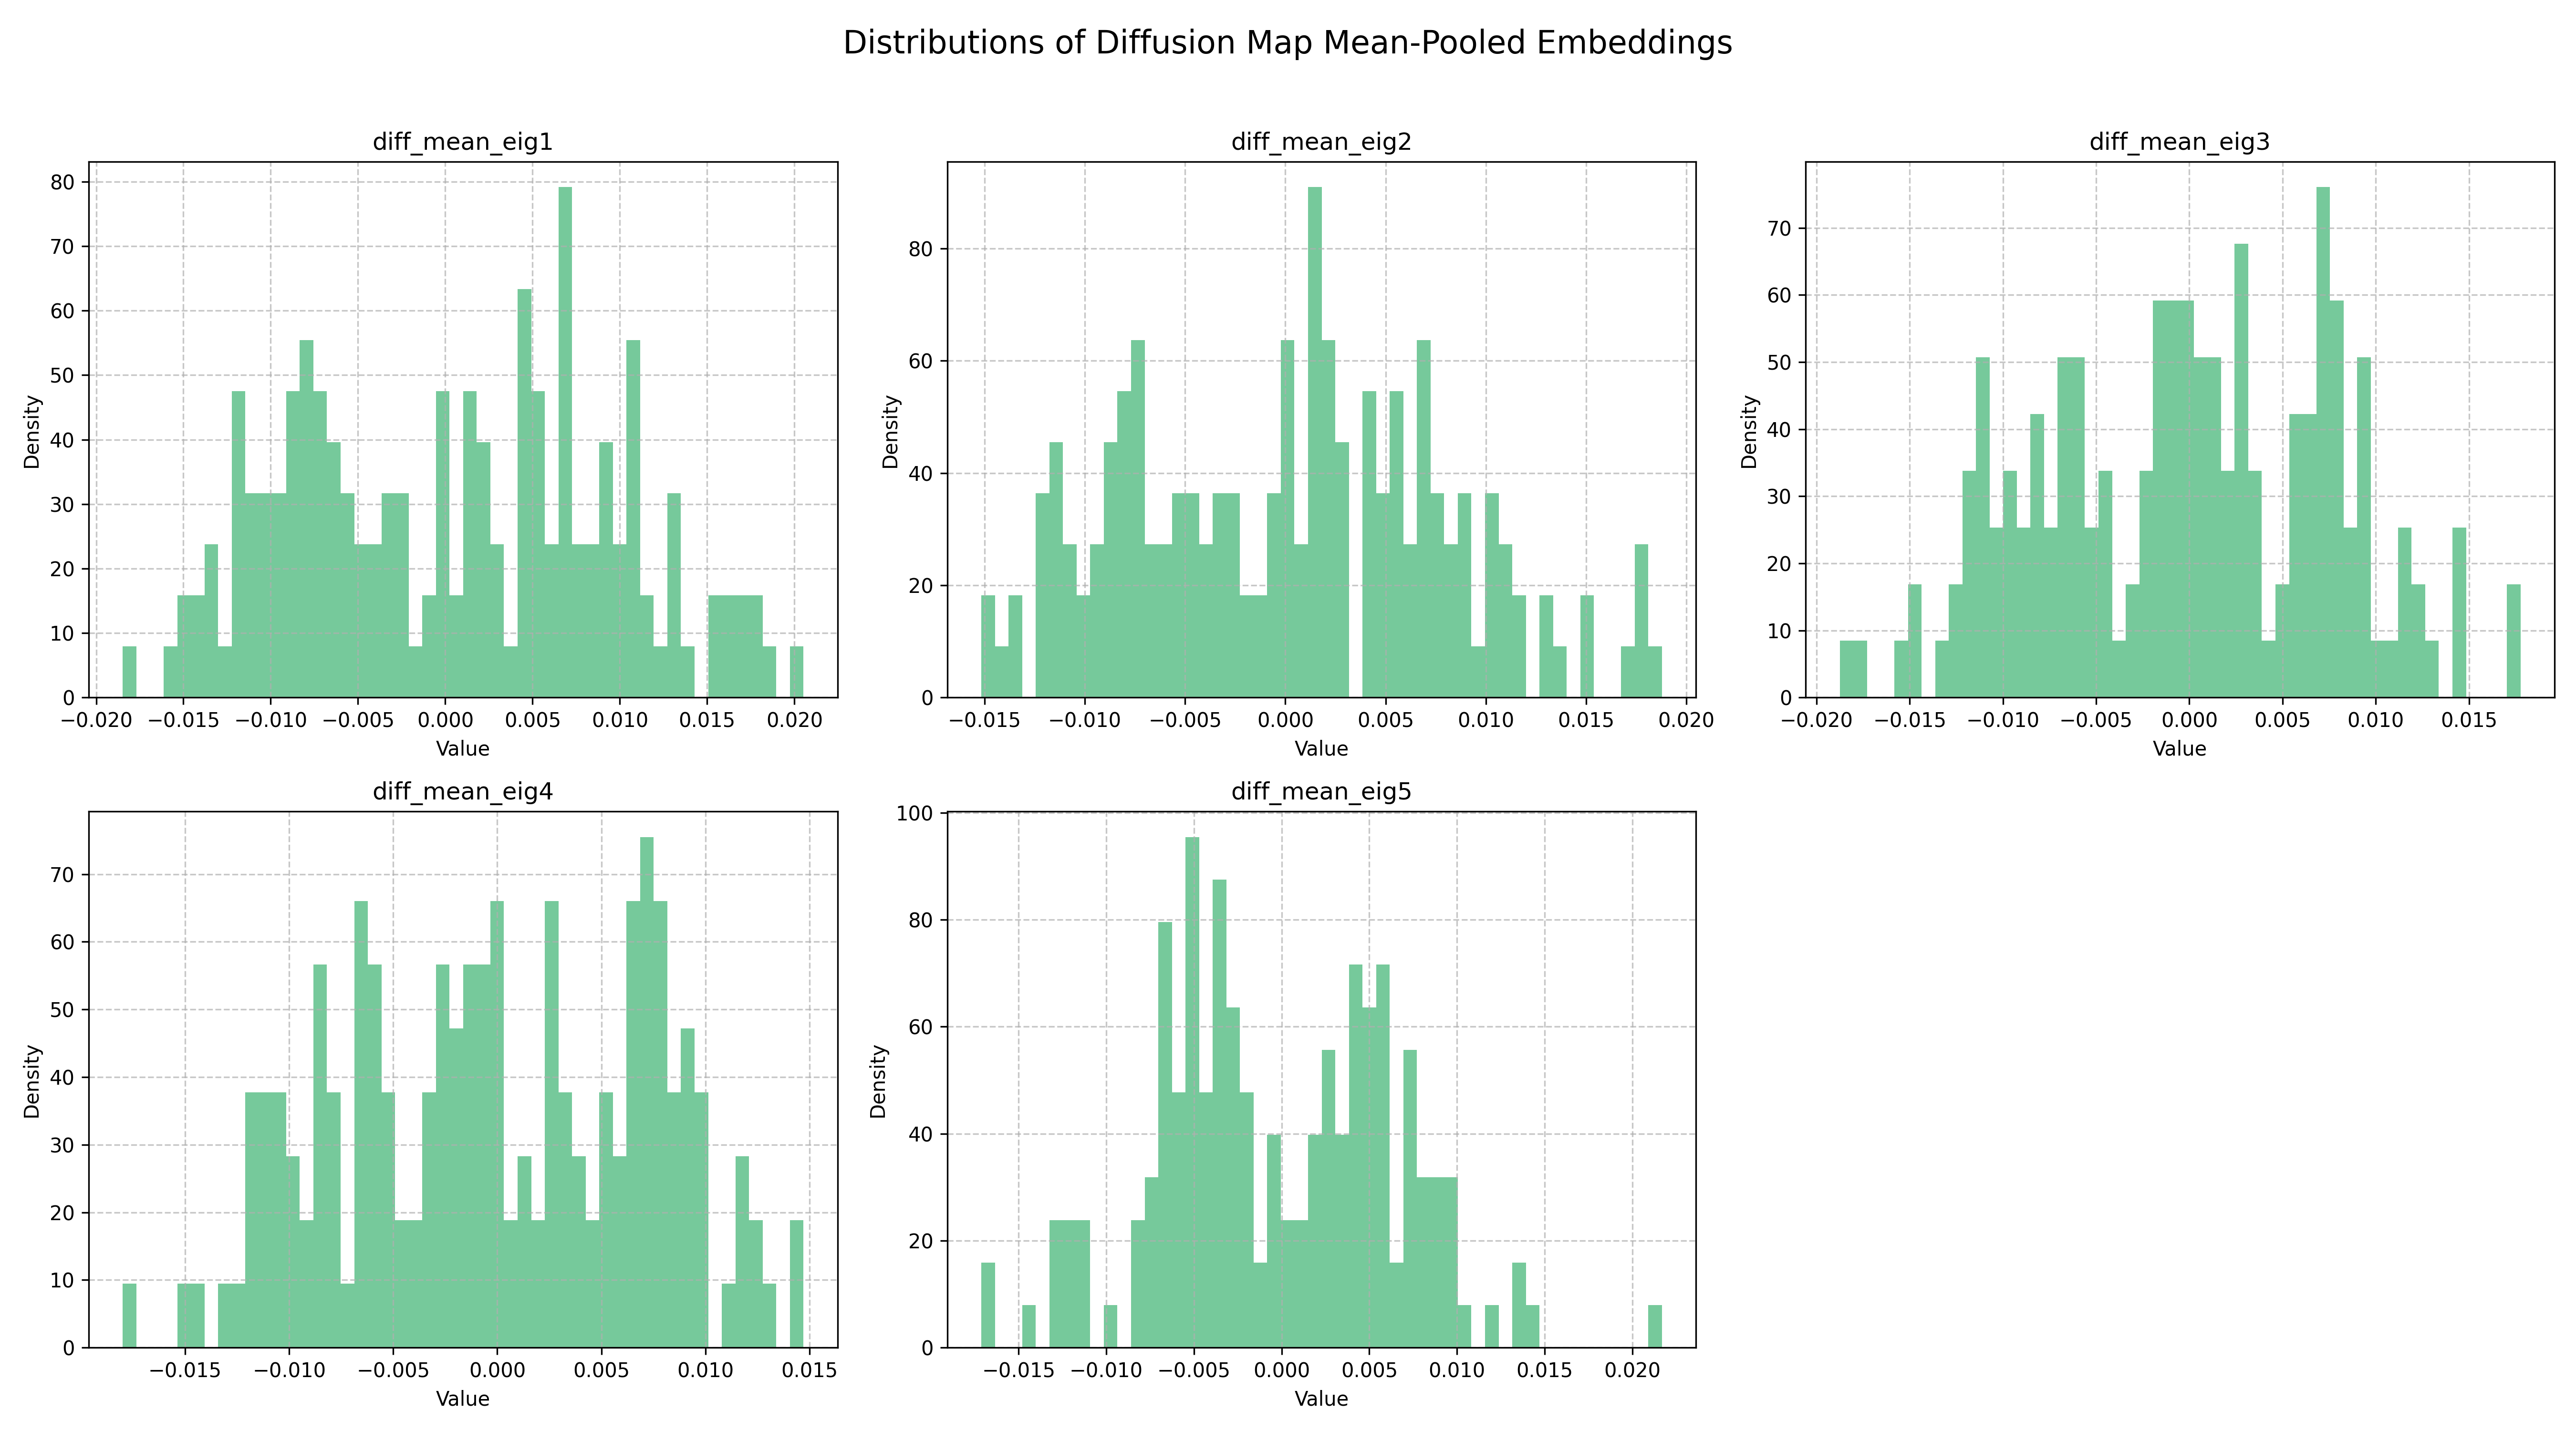
\includegraphics[width=0.5\textwidth]{../input_files/plots/engineered_feature_dist_diff_mean_3_20250527-135752.png}
    \caption{Histograms showing the distributions of the mean-pooled embeddings from the top 5 eigenvectors of the diffusion map. These features, computed on merger trees and imputed for large graphs, were intended to capture structural information, but ultimately failed to predict cosmological parameters.}
    \label{fig:diffusion_feature_dist_mean}
\end{figure}

\begin{figure}[h!]
    \centering
    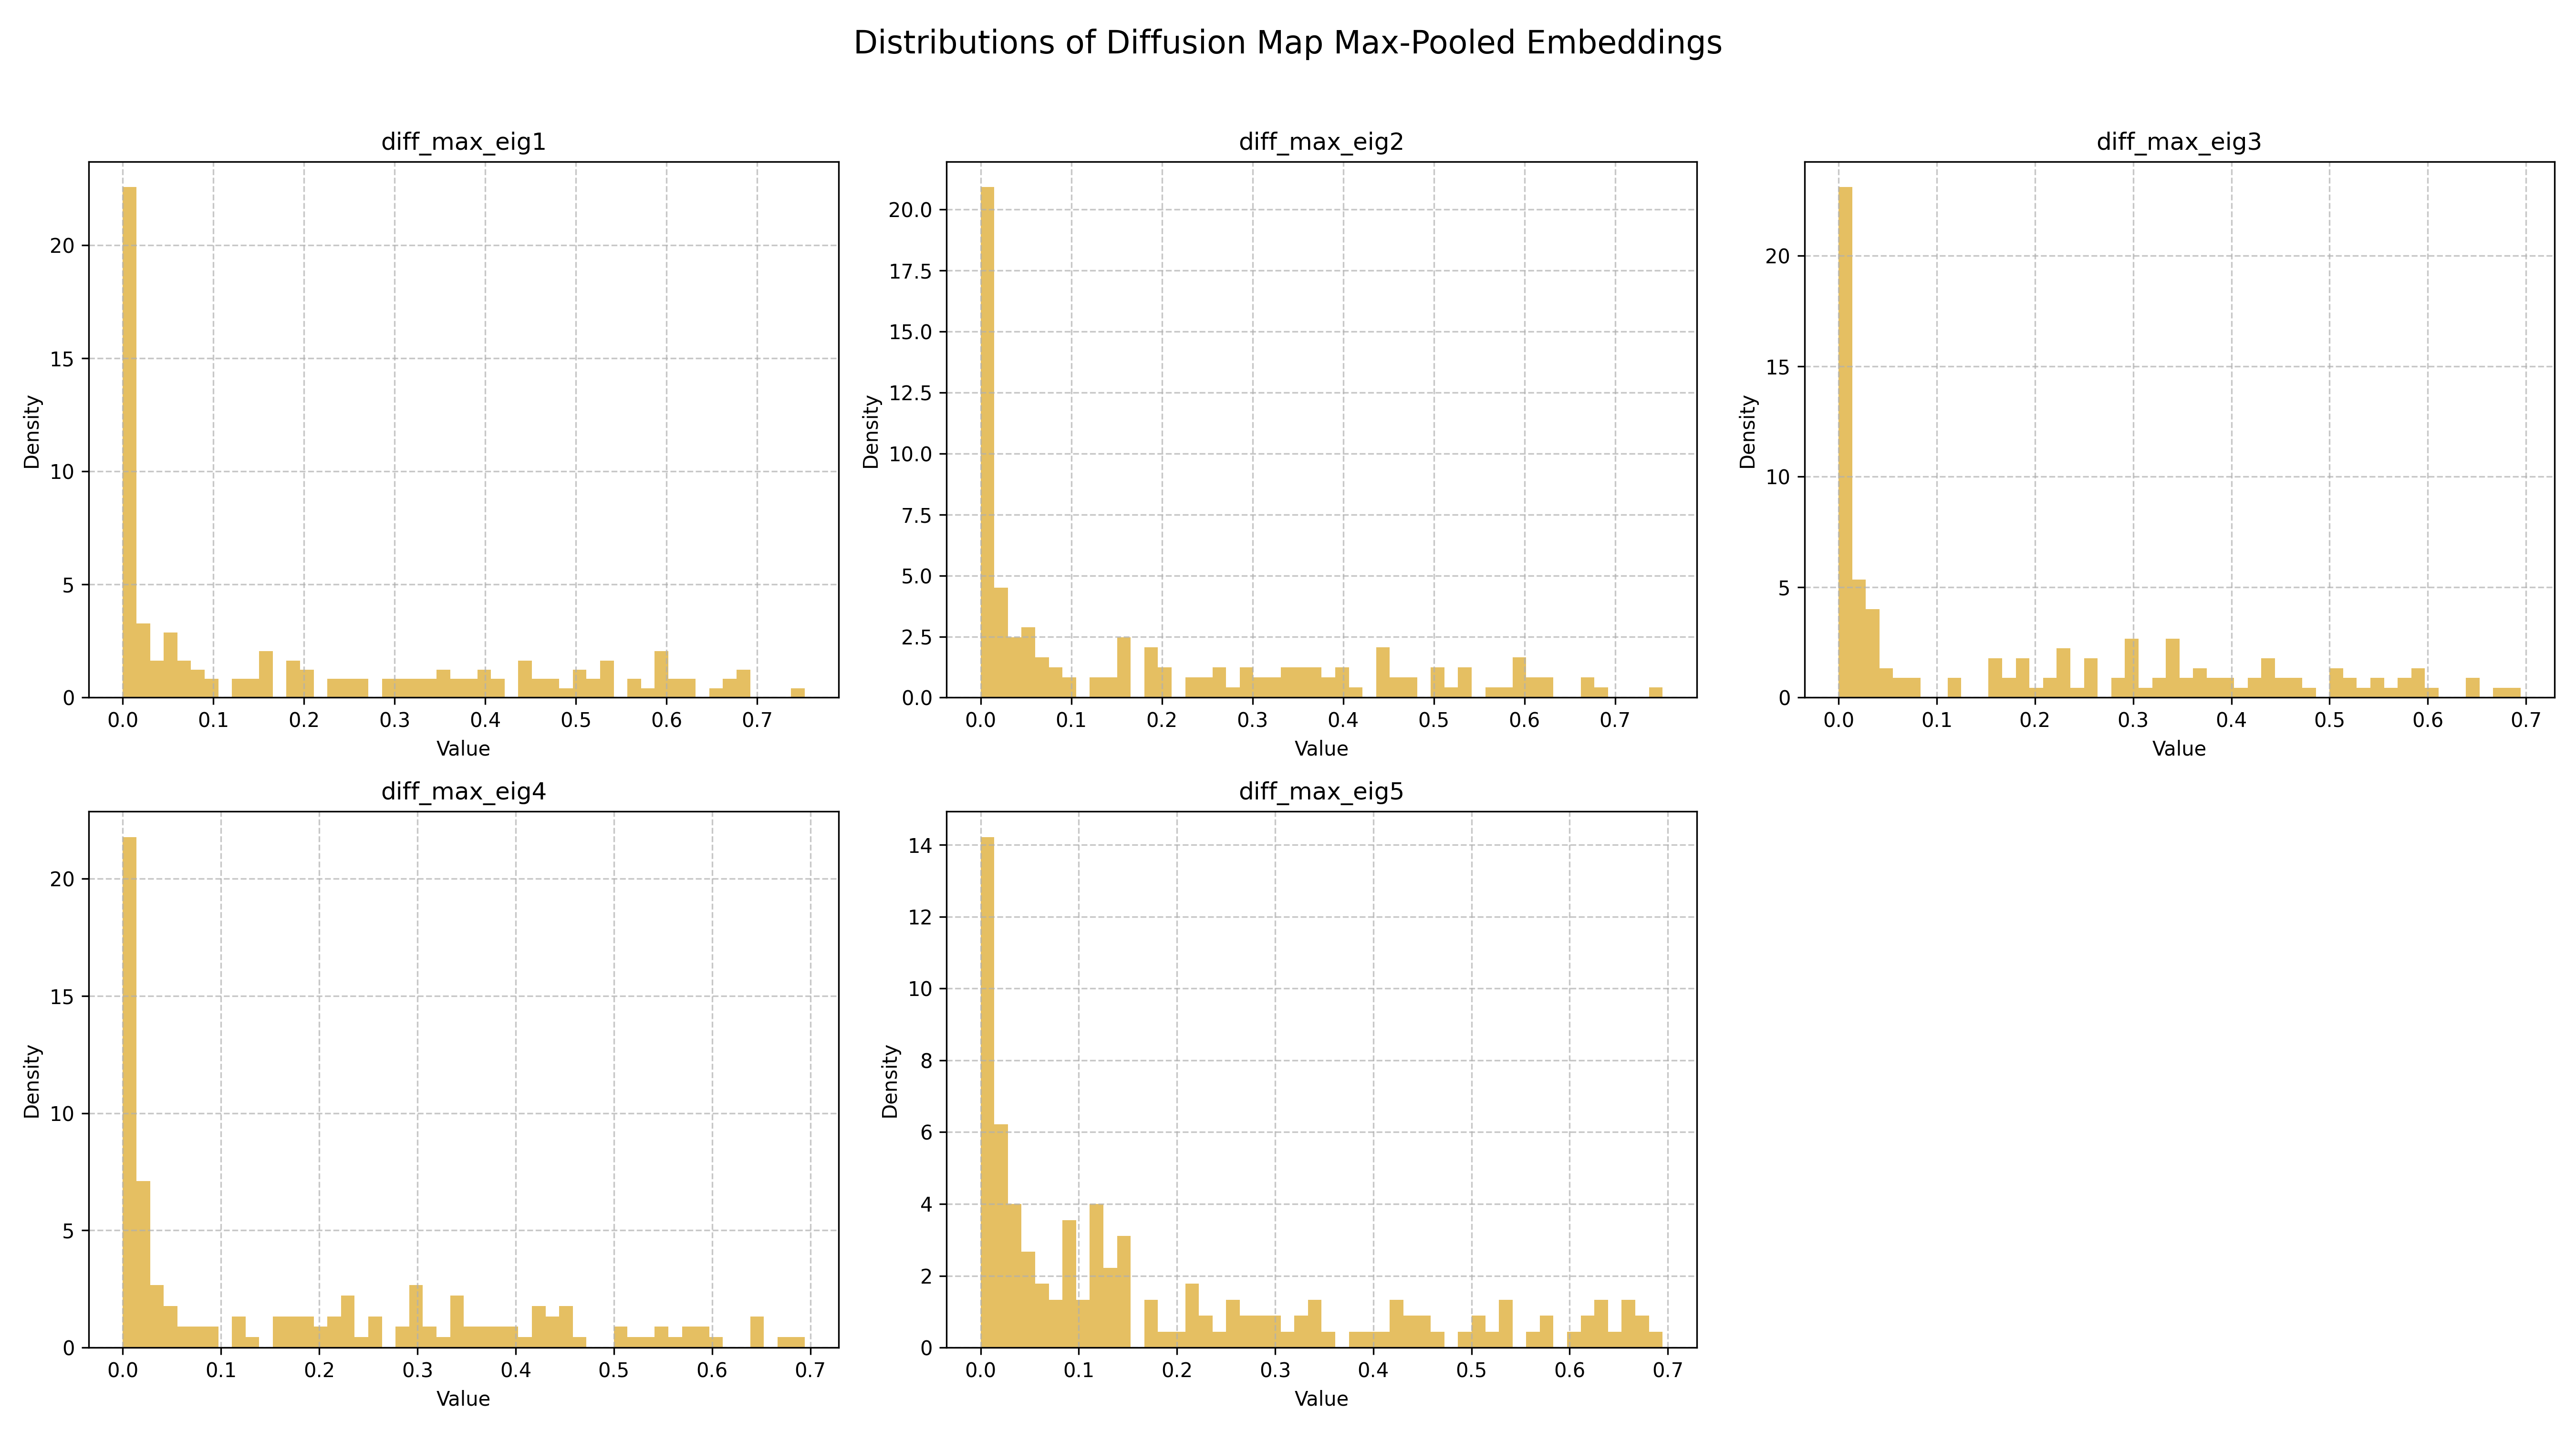
\includegraphics[width=0.5\textwidth]{../input_files/plots/engineered_feature_dist_diff_max_4_20250527-135752.png}
    \caption{Distributions of the max-pooled diffusion map embeddings, showing the feature distributions after mean imputation of NaN values resulting from computational constraints for large graphs. These features did not prove effective in predicting cosmological parameters.}
    \label{fig:diffusion_feature_dist}
\end{figure}

\begin{figure}[h!]
    \centering
    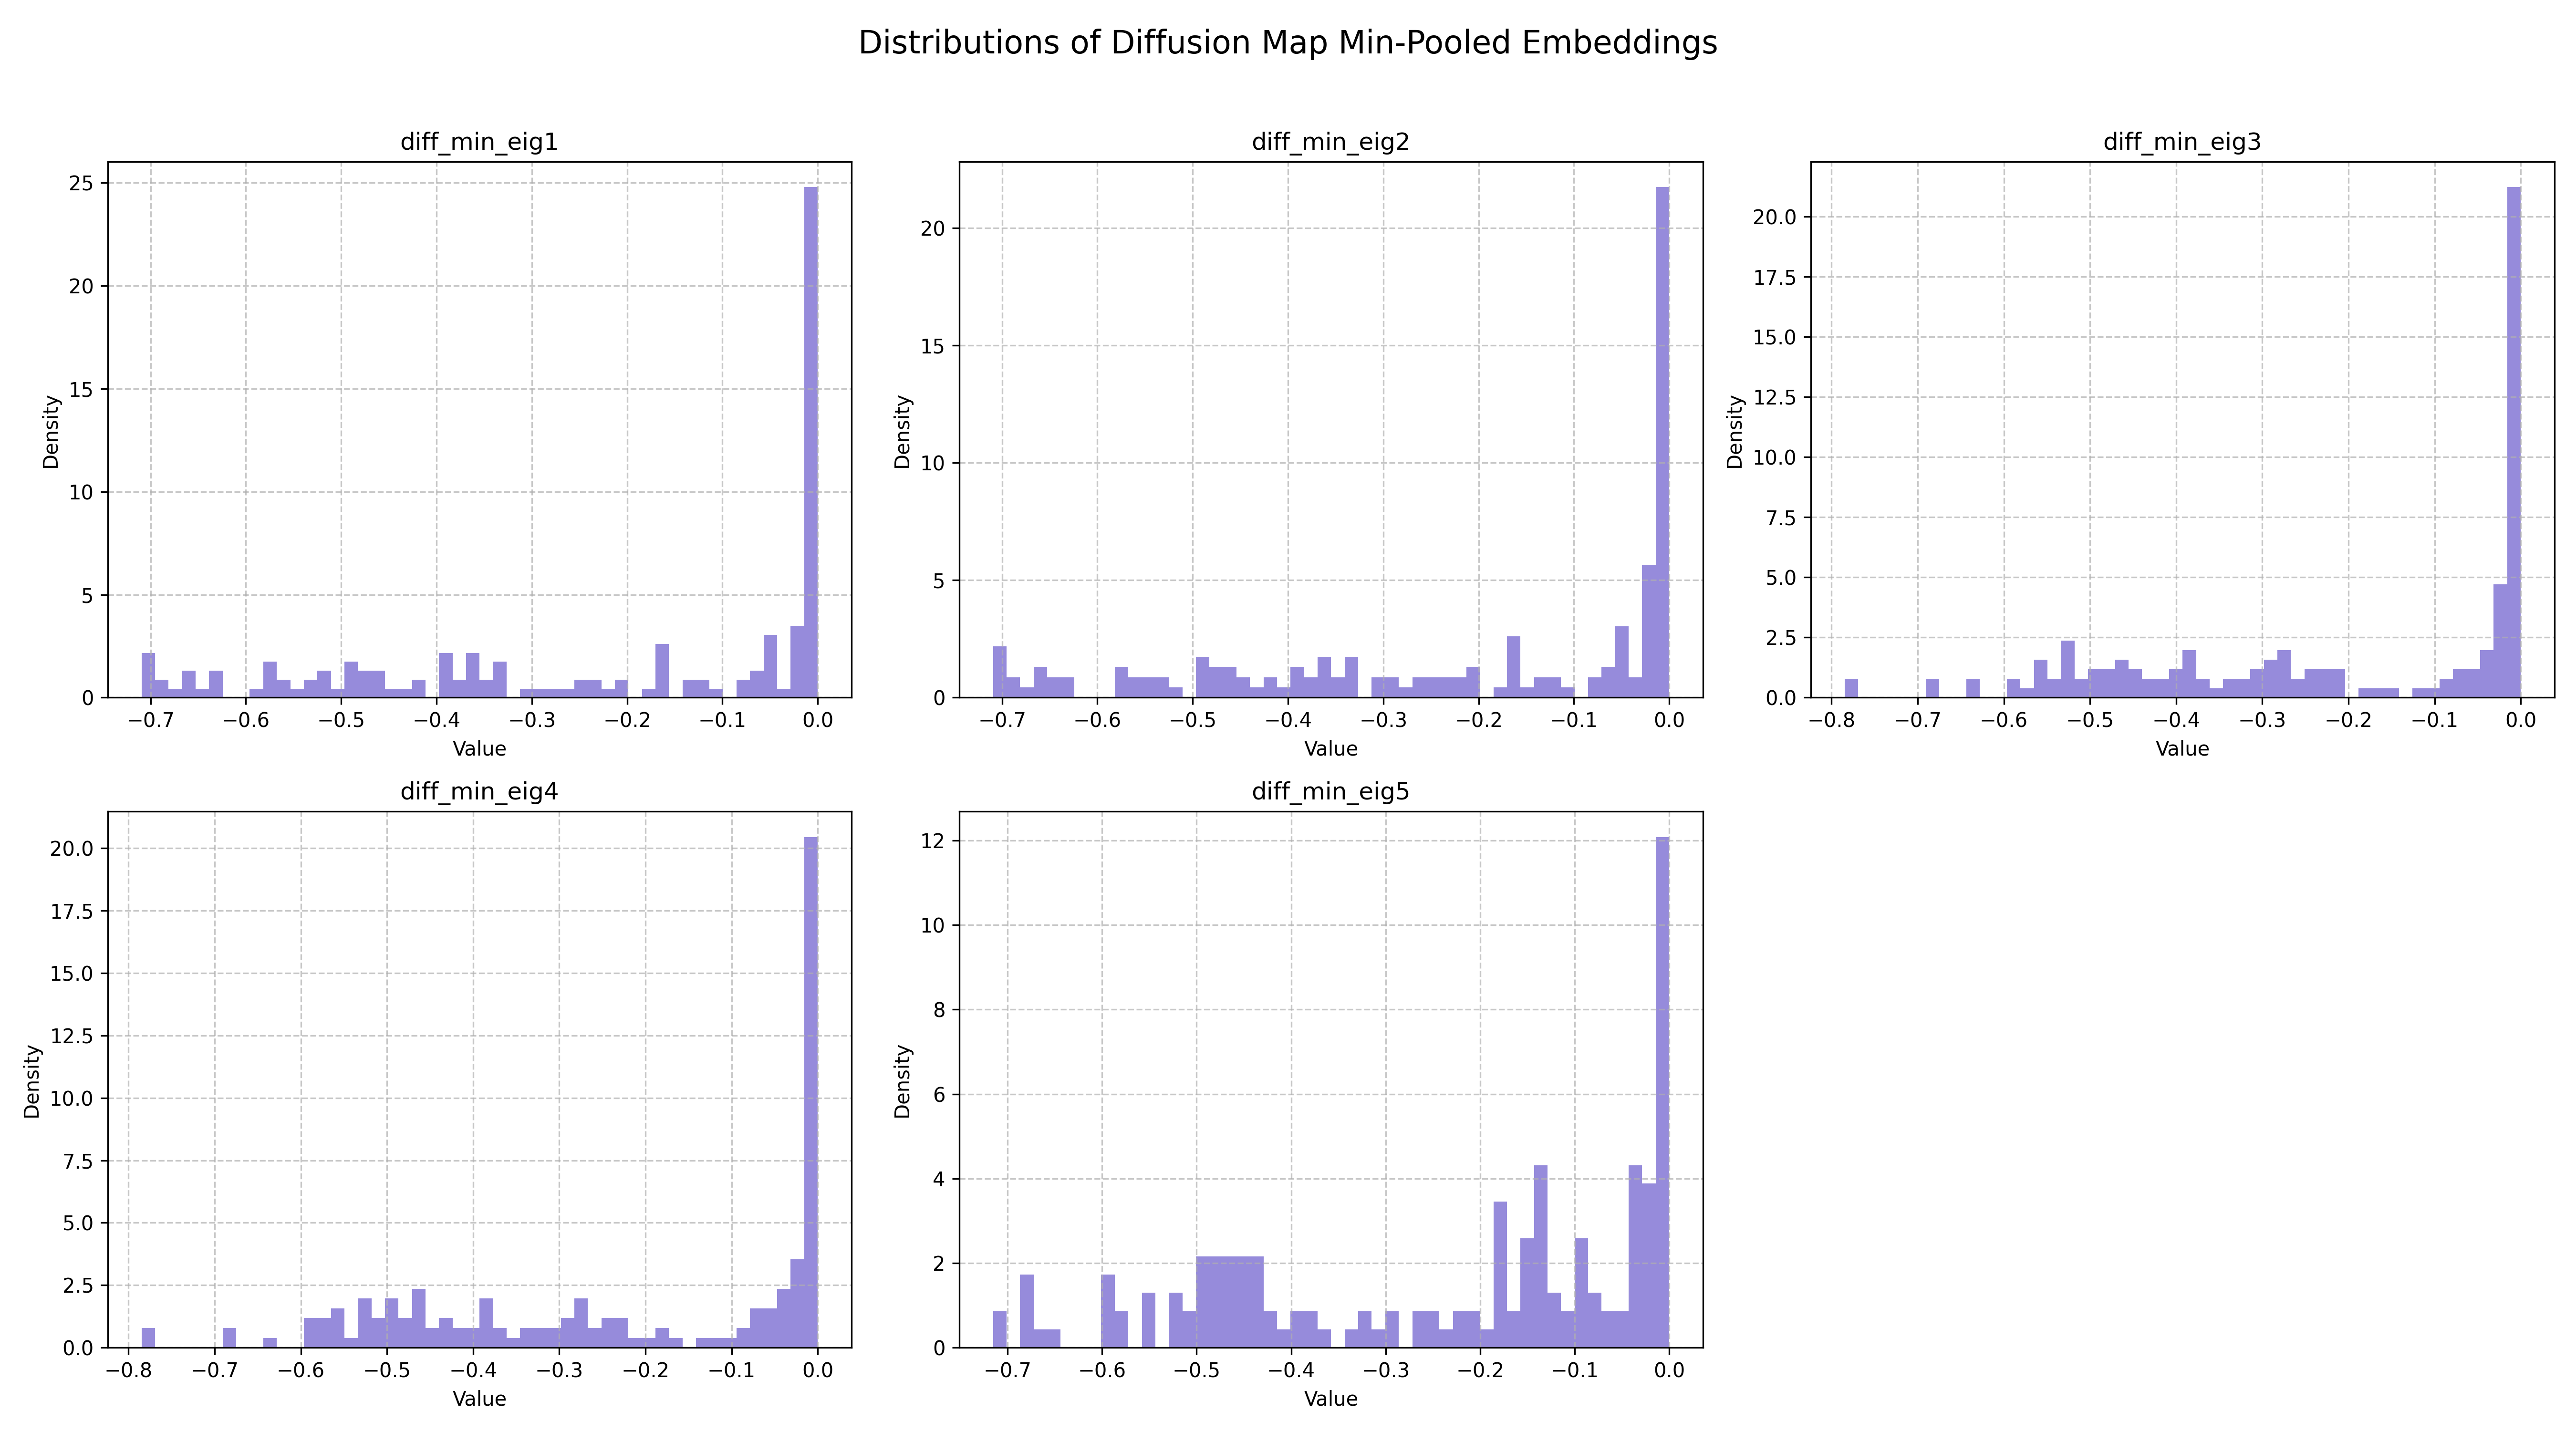
\includegraphics[width=0.5\textwidth]{../input_files/plots/engineered_feature_dist_diff_min_5_20250527-135752.png}
    \caption{Histograms showing the distribution of the minimum-pooled diffusion map embeddings for the first five eigenvectors, illustrating the impact of imputing NaN values due to computational constraints during feature engineering, which likely contributed to the poor performance of these features in predicting cosmological parameters.}
    \label{fig:diffusion_feature_dist_min}
\end{figure}

\subsection{Dimensionality Reduction of Engineered Features}

To reduce dimensionality and decorrelate features, Principal Component Analysis (PCA) was applied to the mean-imputed 24 engineered features derived from the training set. The goal was to retain most of the variance while reducing the number of features. The PCA explained variance plot (available in `data/pca\_explained\_variance\_plot\_1_<timestamp>.png`) shows the cumulative and individual explained variance per component. Based on this analysis, it was determined that 8 principal components were sufficient to explain approximately 96.29\% of the variance in the engineered feature space. Consequently, both training and test engineered feature sets were transformed into this 8-dimensional PCA space.

\begin{figure}[h!]
    \centering
    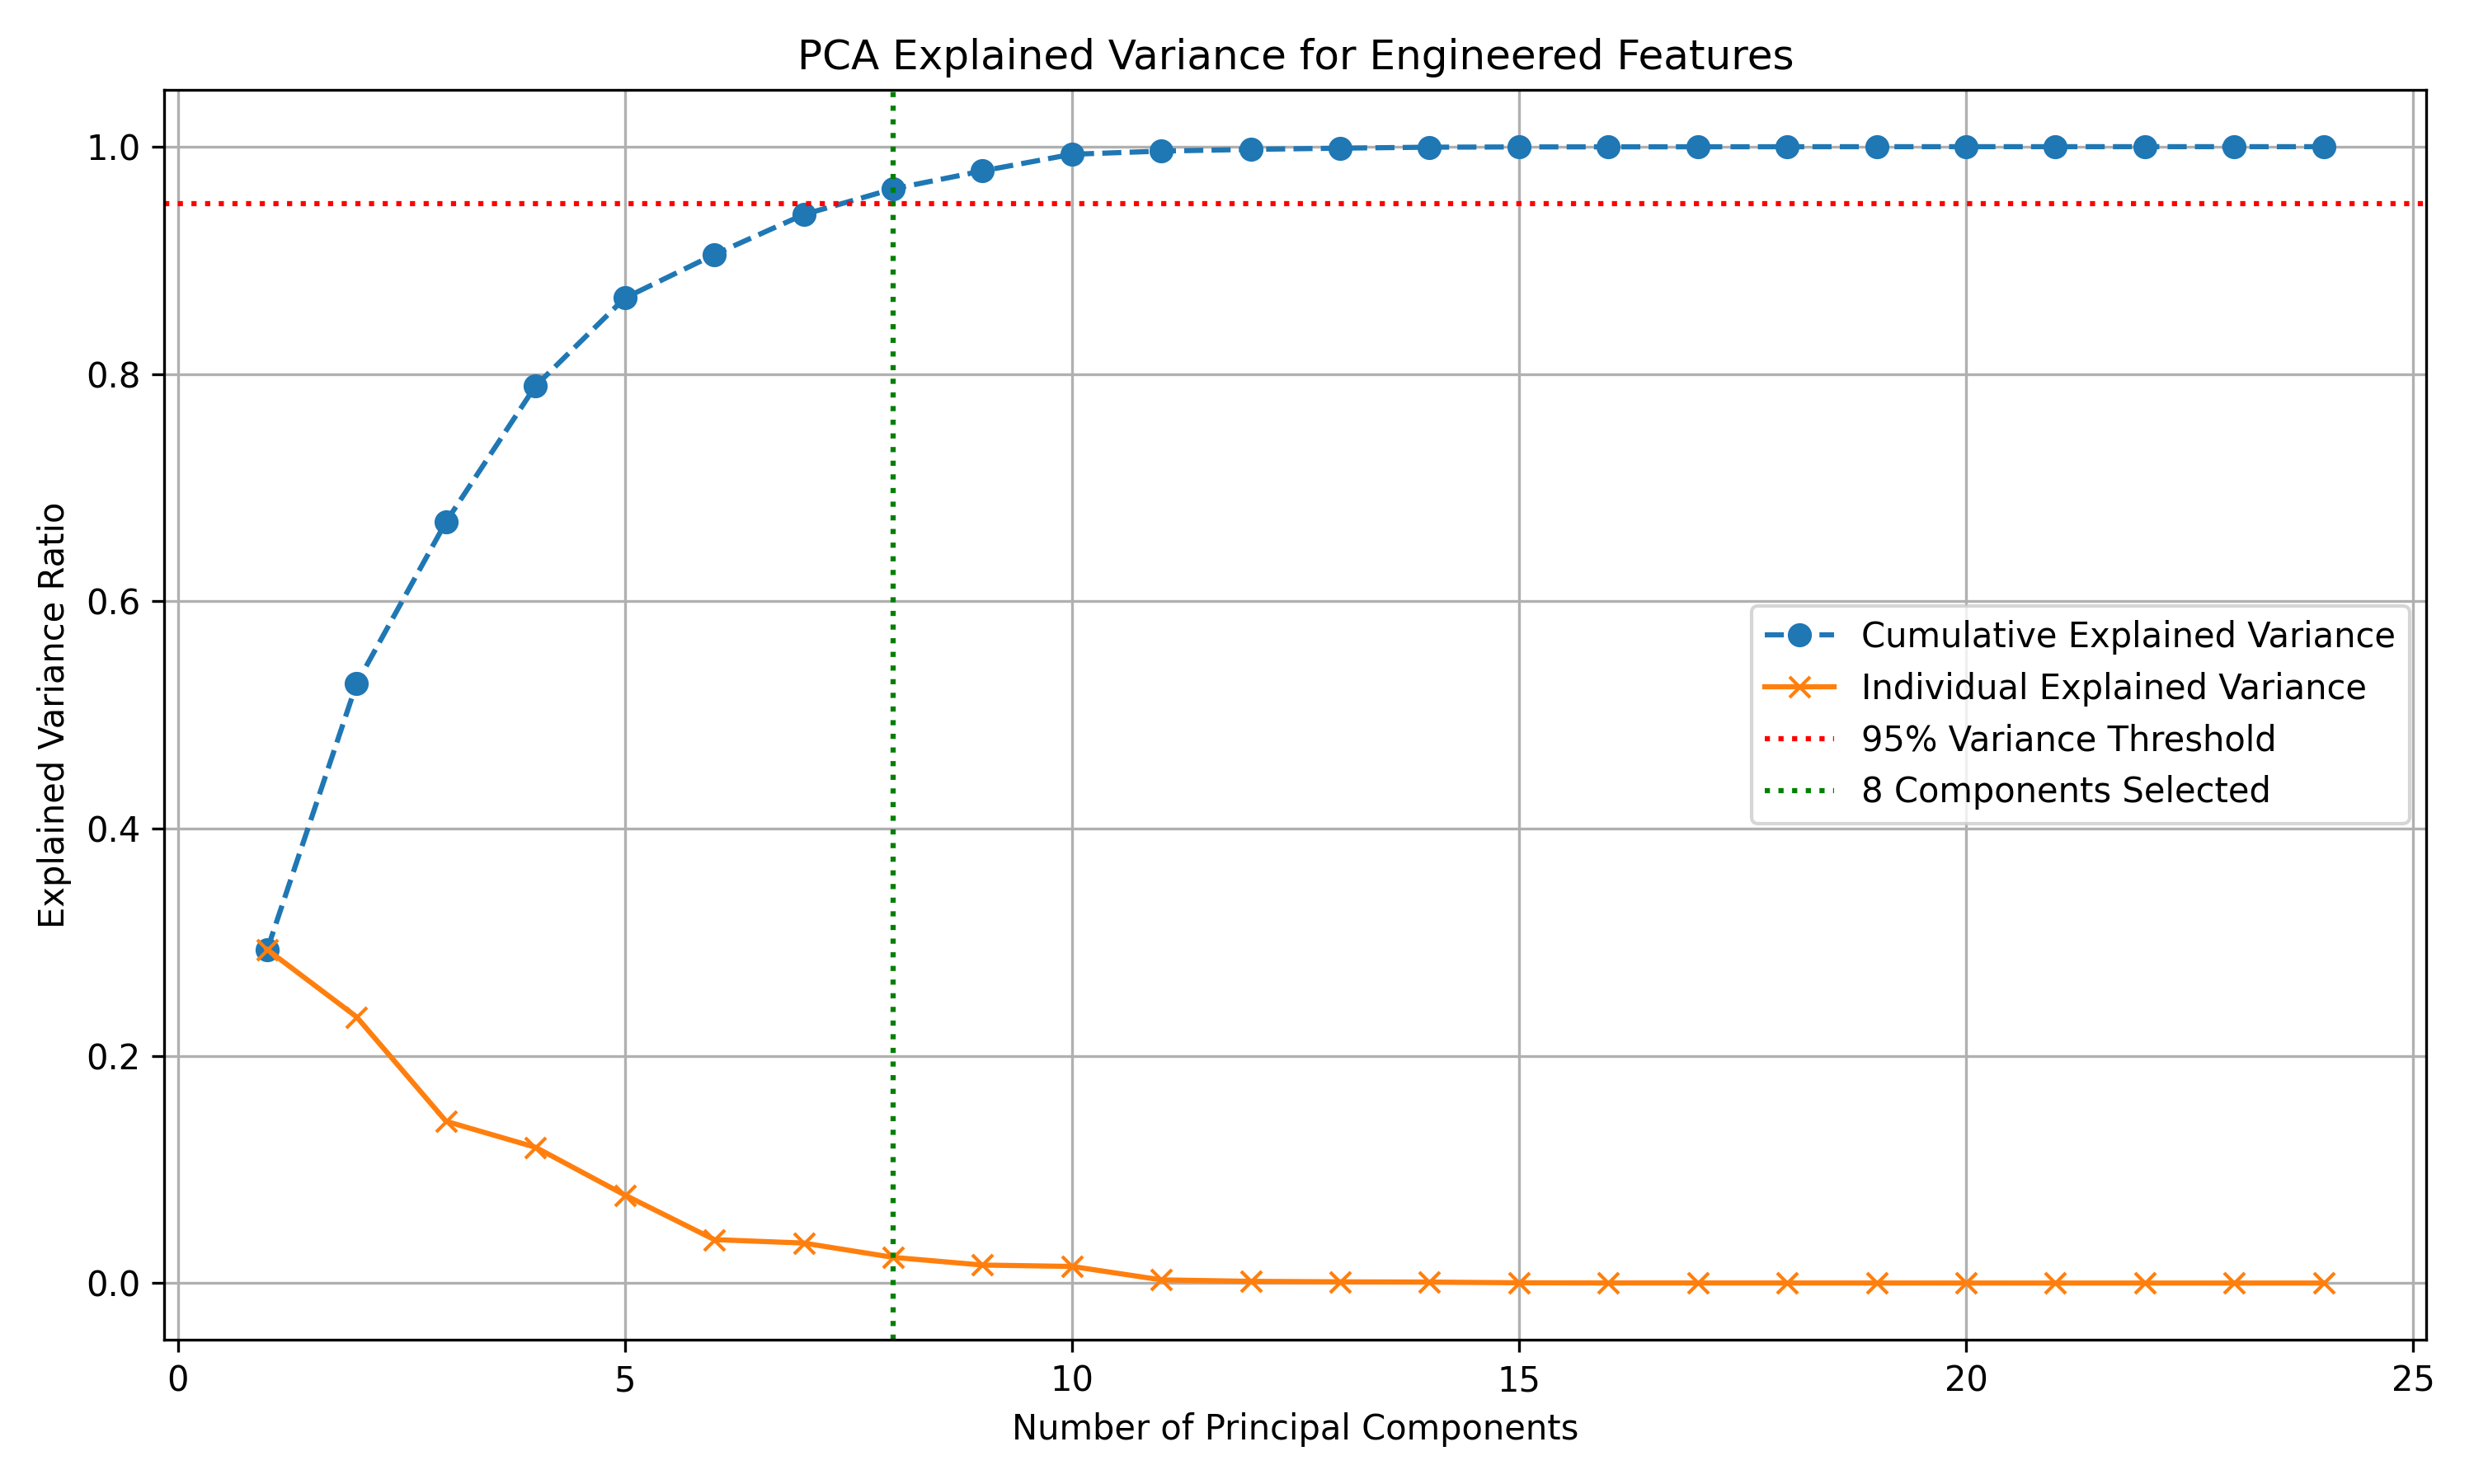
\includegraphics[width=0.5\textwidth]{../input_files/plots/pca_explained_variance_plot_1_20250527-134016.png}
    \caption{PCA explained variance plot for engineered features. Eight principal components were sufficient to explain 96.29\% of the variance. However, models trained on these PCA-transformed features performed poorly, suggesting that the retained variance did not capture information relevant for predicting cosmological parameters.}
    \label{fig:pca_explained_variance}
\end{figure}

To visualize the PCA-transformed data, scatter plots of the first two principal components (PC1 vs. PC2) were generated, colored by the true values of $\Omega_m$ and $\sigma_8$ (available in `data/pca\_projection\_plot\_6_<timestamp>.png`). These projections did not reveal any immediately obvious strong linear separation or clear clustering of data points corresponding to different $\Omega_m$ or $\sigma_8$ values. The points were largely intermingled, suggesting that the first two principal components of the engineered features may not linearly capture strong cosmological signatures in a visually separable manner. This lack of clear visual separation hints that the relationship between the engineered features (even after PCA) and the cosmological parameters might be complex, non-linear, or that these features are not strongly discriminative.

\begin{figure}[h!]
    \centering
    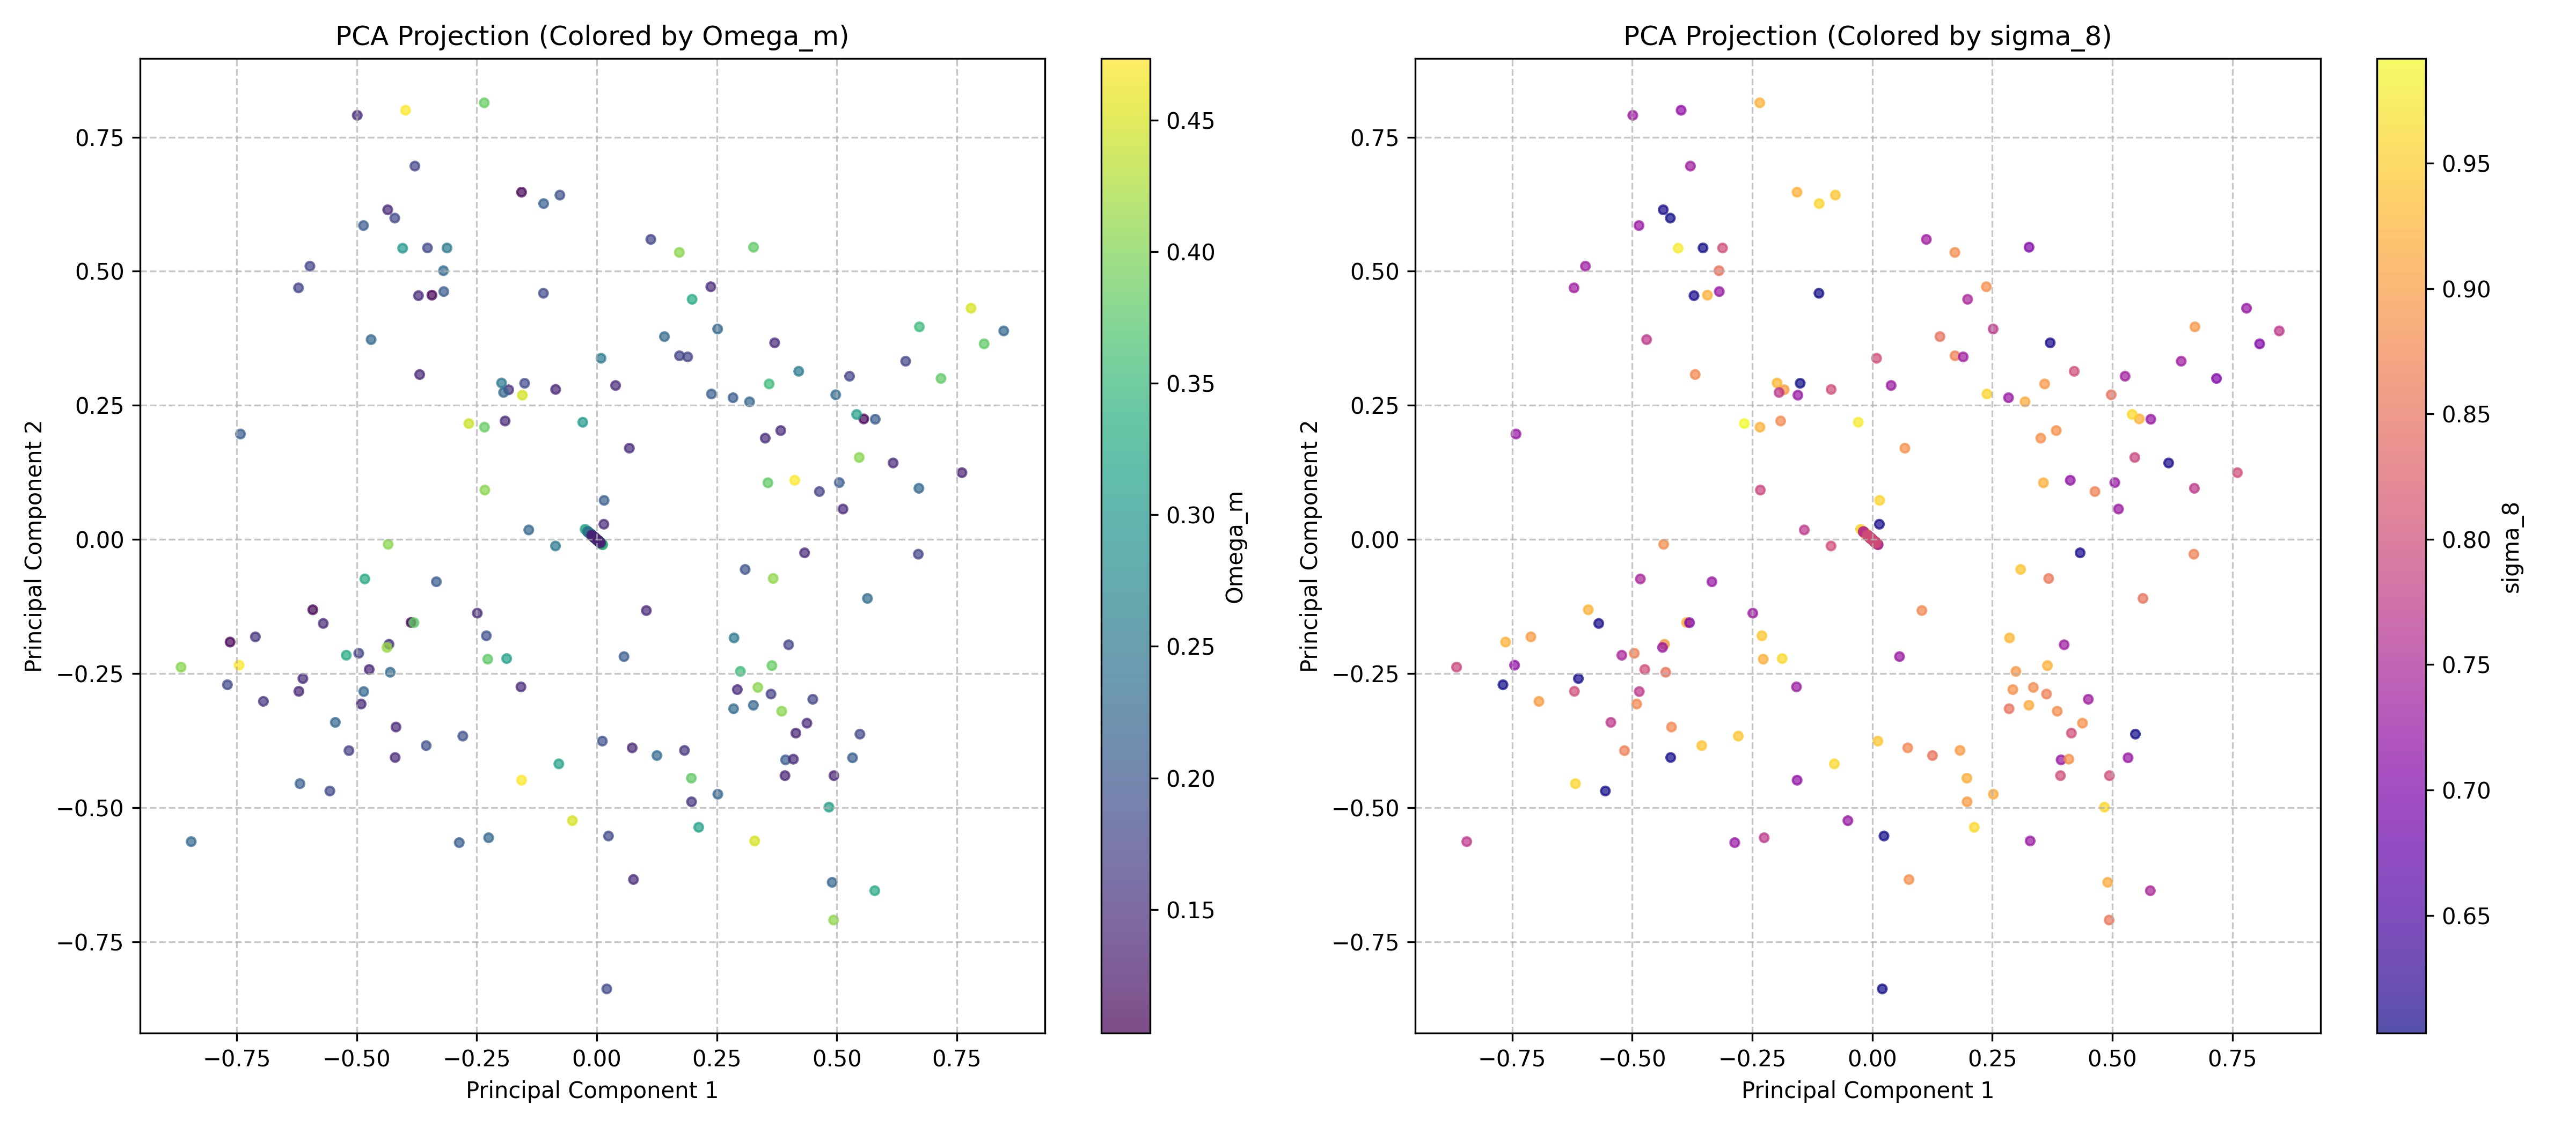
\includegraphics[width=0.5\textwidth]{../input_files/plots/pca_projection_plot_6_20250527-135752.png}
    \caption{Scatter plots of the first two principal components of the engineered features, colored by $\Omega_m$ (left) and $\sigma_8$ (right). There is no clear visual separation between different values of the cosmological parameters.}
    \label{fig:pca_projection}
\end{figure}

\subsection{Baseline Feature Sets}

Two baseline approaches were established for comparison:
\begin{enumerate}
    \item Baseline Aggregated Node Features: For each graph, 16 features were computed by taking the mean, standard deviation, minimum, and maximum of each of the 4 normalized node features across all nodes in that graph. These features provide simple global statistics of the halo properties within each merger tree. No NaNs were present in these baseline features after computation.
    \item Graph Convolutional Network (GCN): A GCN model was implemented for graph-level regression. It consisted of two `GCNConv` layers with ReLU activations, followed by a global mean pooling layer and two fully connected layers for regression. The GCN was trained on normalized node features and graph structures for 50 epochs on a CPU.
\end{enumerate}

\subsection{Predictive Performance of Cosmological Parameters}

Regression models (Random Forest Regressor - RFR, Gradient Boosting Regressor - GBR) were trained on both the PCA-transformed engineered features and the baseline aggregated node features. The GCN provided a deep learning baseline. Performance was evaluated using R-squared (R²) and Mean Squared Error (MSE) on the test set. All hyperparameters for RFR and GBR were tuned using `GridSearchCV` with `GroupKFold` (5 splits) based on `lh_id` to prevent data leakage.

A summary of the model performances is presented in Table 1.

\begin{table}[h!]
\centering
\caption{Model Performance on Test Set for Predicting $\Omega_m$ and $\sigma_8$}
\begin{tabular}{|l|l|l|l|l|}
\hline
Feature Set             & Model & Target    & R²      & MSE        \\ \hline
Engineered + PCA    & RFR   & $\Omega_m$  & -0.2682 & 0.010926   \\ \hline
                        & GBR   & $\Omega_m$  & -0.1885 & 0.010240   \\ \hline
                        & RFR   & $\sigma_8$  & -0.4622 & 0.016500   \\ \hline
                        & GBR   & $\sigma_8$  & -0.4412 & 0.016262   \\ \hline
Baseline Aggregated & RFR   & $\Omega_m$  & 0.8879  & 0.000966   \\ \hline
                        & GBR   & $\Omega_m$  & 0.9134  & 0.000746   \\ \hline
                        & RFR   & $\sigma_8$  & 0.2827  & 0.008094   \\ \hline
                        & GBR   & $\sigma_8$  & 0.4238  & 0.006502   \\ \hline
GCN                     & GCN   & $\Omega_m$  & 0.9786  & 0.000185   \\ \hline
                        & GCN   & $\sigma_8$  & 0.4977  & 0.005668   \\ \hline
\end{tabular}
\label{tab:model_performance}
\end{table}

The visualizations of the performance comparison (available in `data/model\_performance\_r2\_11_<timestamp>.png` for R² and `data/model\_performance\_mse\_12_<timestamp>.png` for MSE) further illustrate these results.

\begin{figure}[h!]
    \centering
    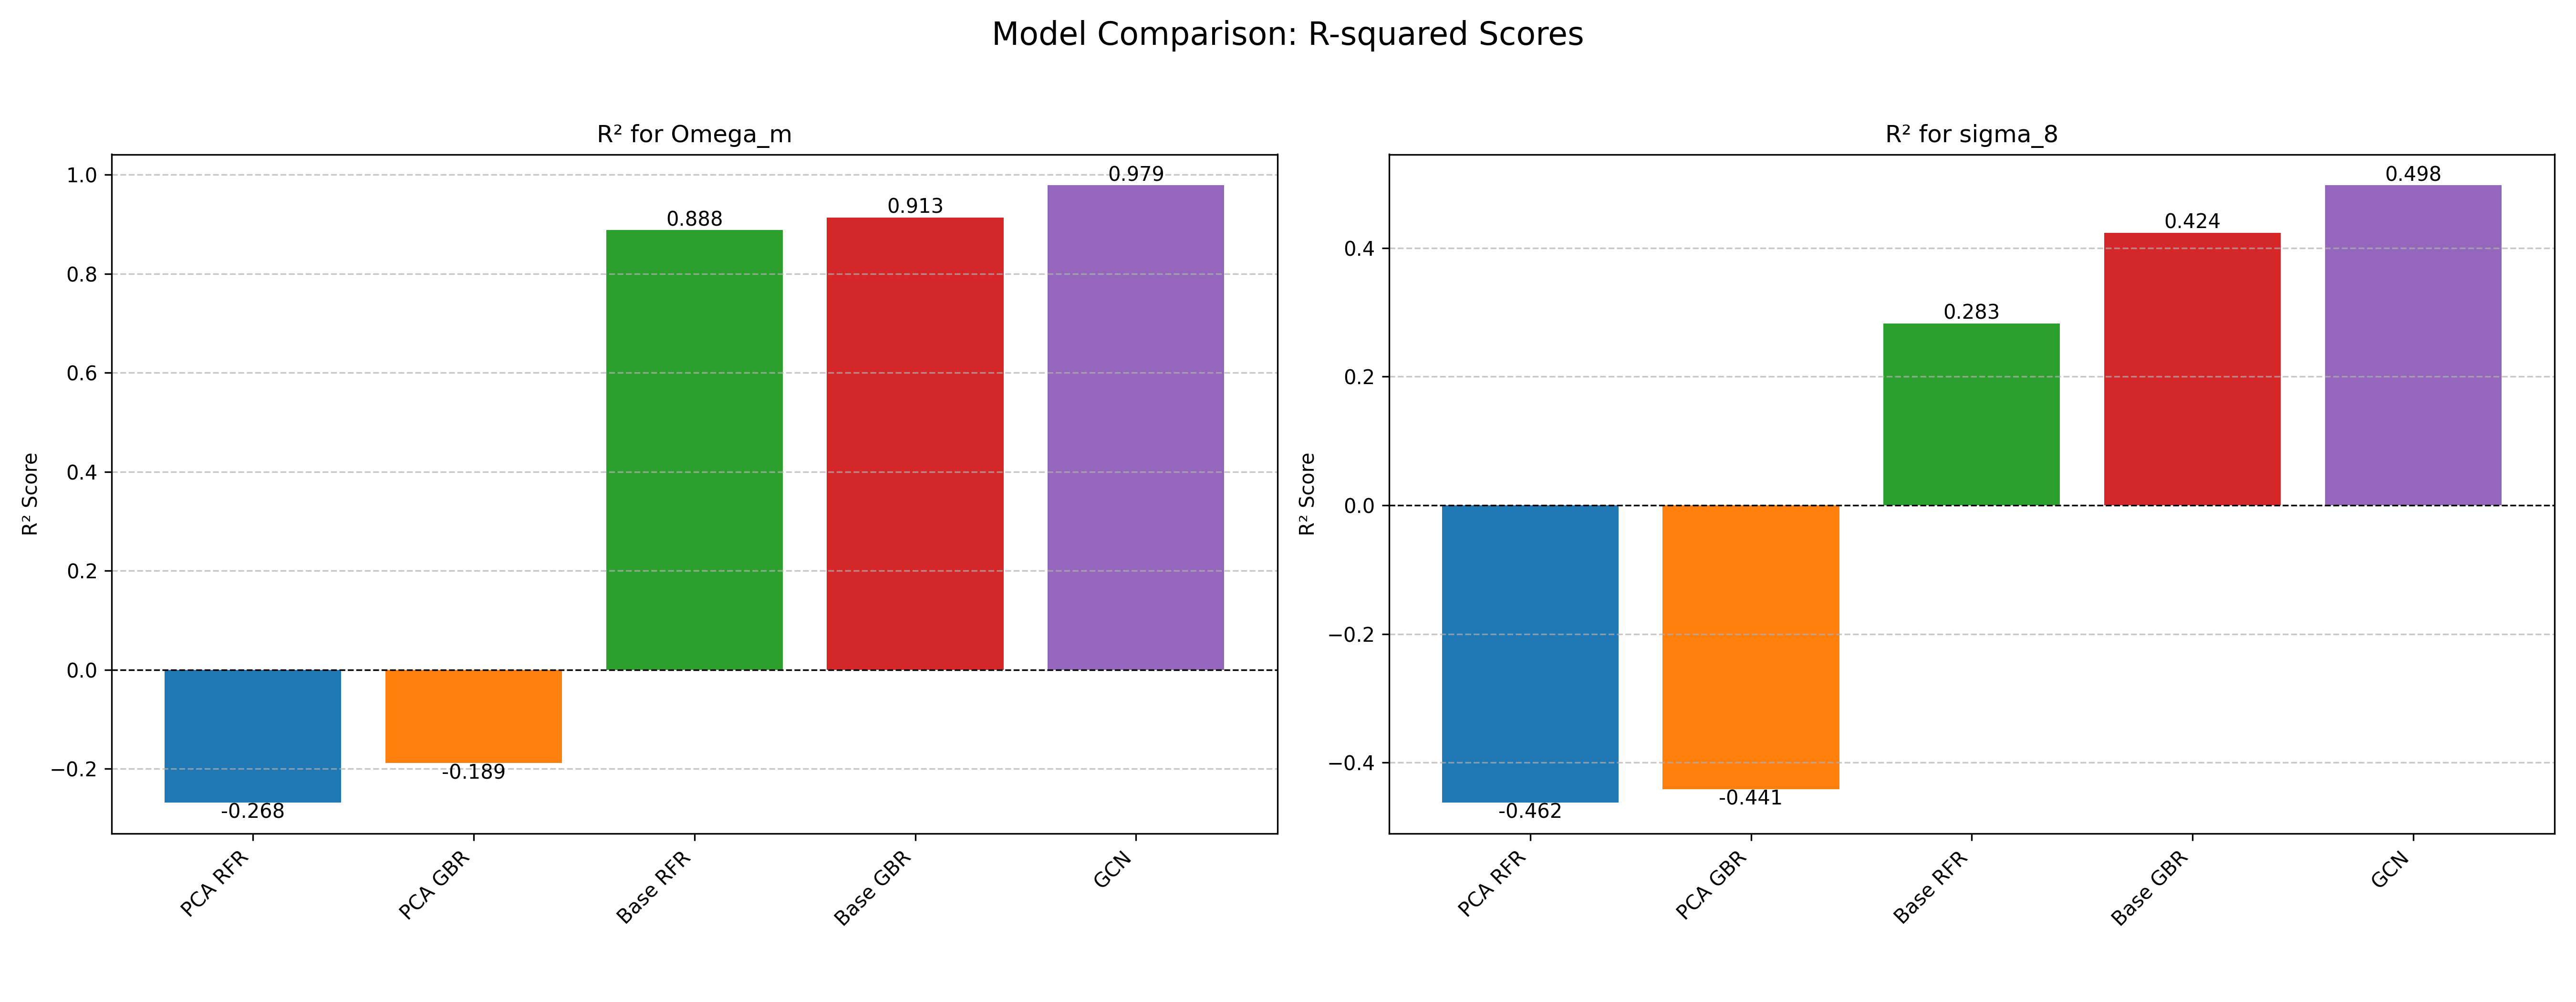
\includegraphics[width=0.5\textwidth]{../input_files/plots/model_performance_r2_11_20250527-135752.png}
    \caption{Comparison of R-squared (R²) scores for predicting $\Omega_m$ and $\sigma_8$ using different feature sets and models. The GCN and baseline aggregated node features outperform engineered features with PCA, which show negative R² values, indicating poor performance.}
    \label{fig:model_performance_r2}
\end{figure}

\begin{figure}[h!]
    \centering
    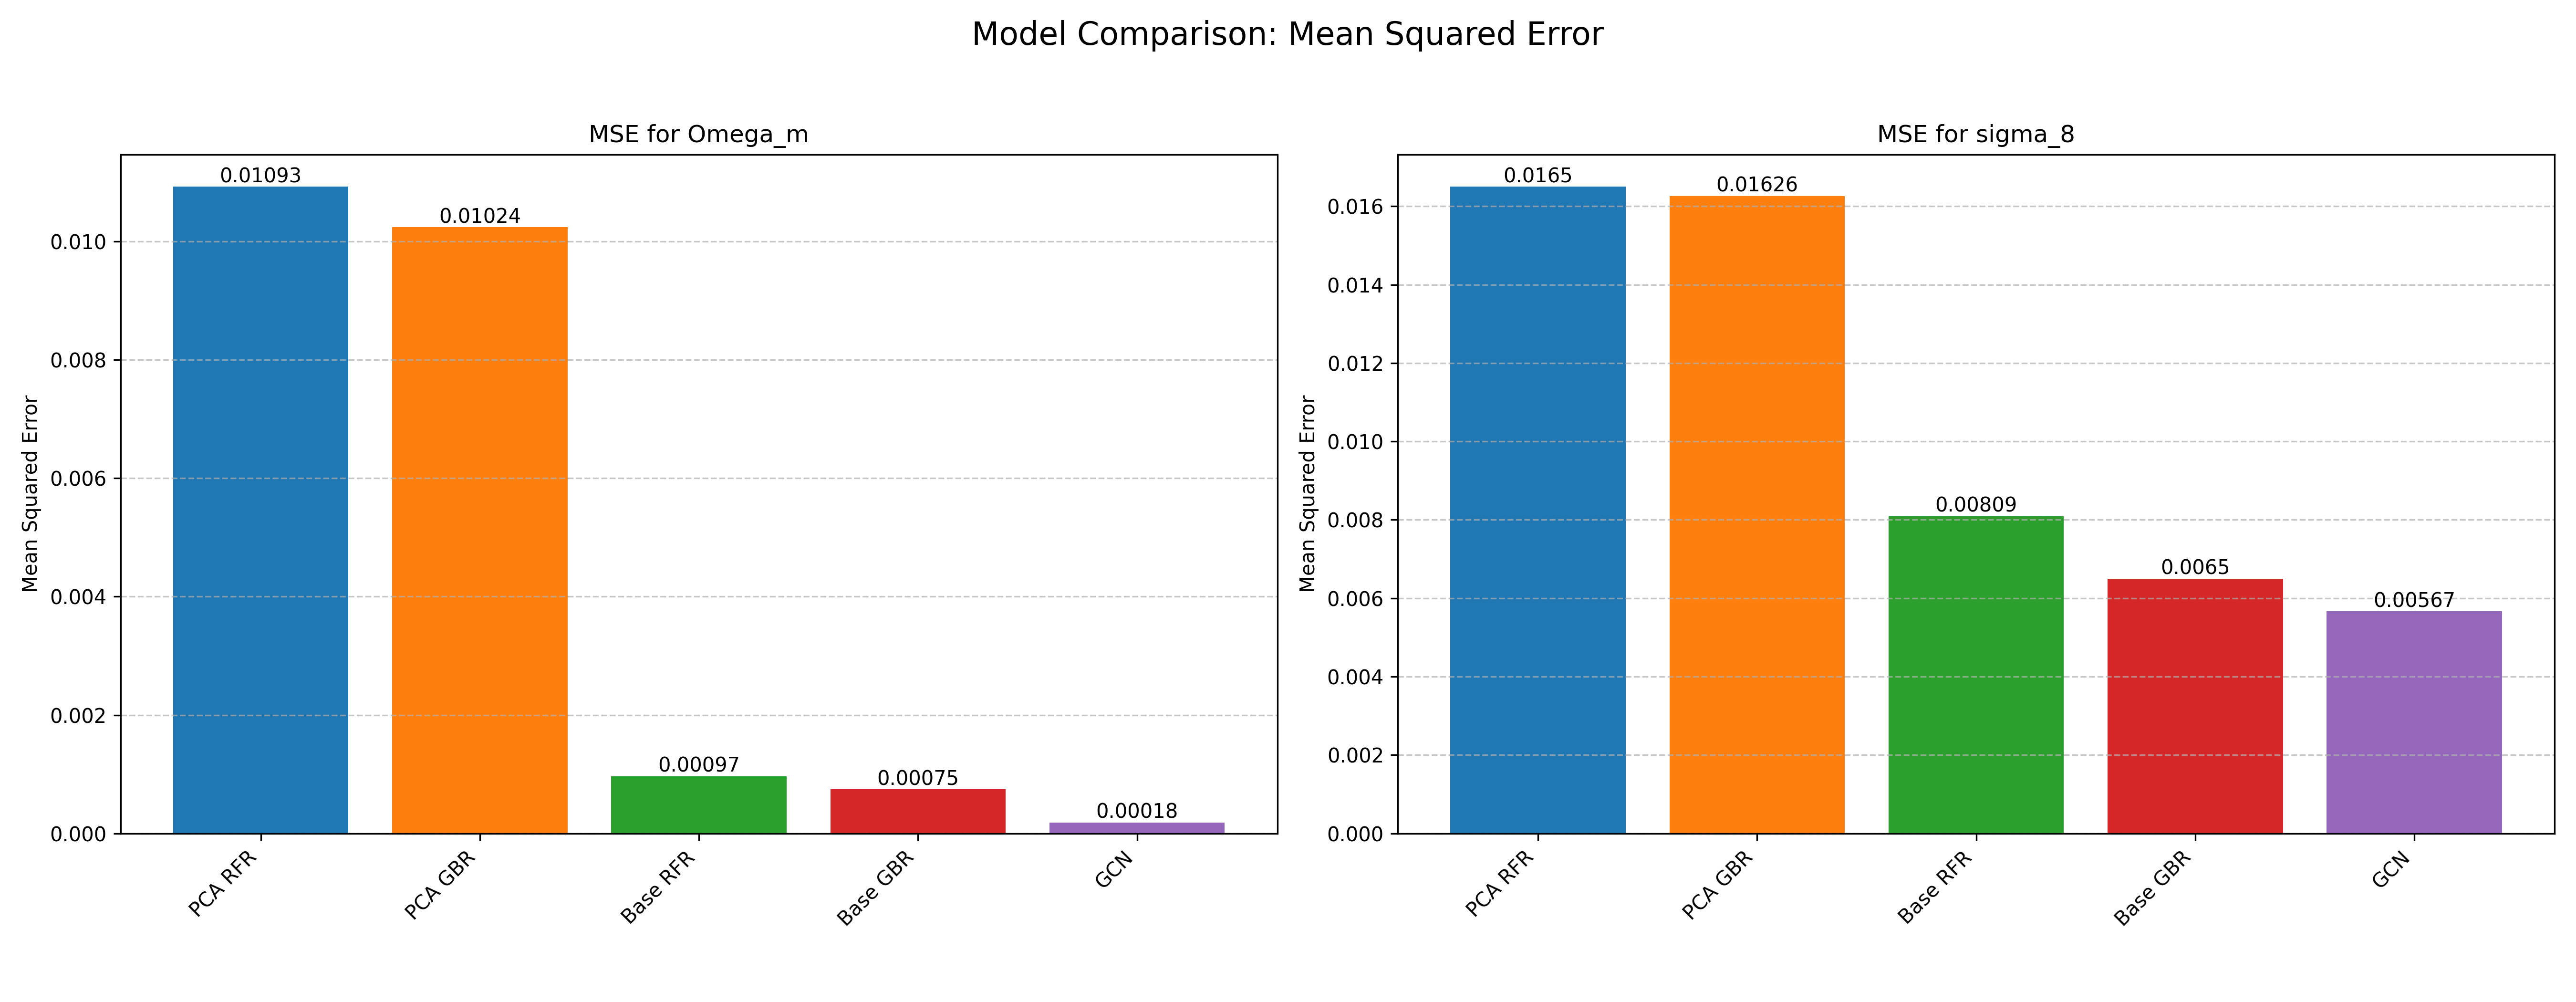
\includegraphics[width=0.5\textwidth]{../input_files/plots/model_performance_mse_12_20250527-135752.png}
    \caption{Mean Squared Error (MSE) comparison of different models (PCA-transformed engineered features with Random Forest Regressor (RFR) and Gradient Boosting Regressor (GBR), baseline aggregated node features with RFR and GBR, and Graph Convolutional Network (GCN)) for predicting $\Omega_m$ and $\sigma_8$. The baseline aggregated node features and the GCN model significantly outperform the engineered features after PCA.}
    \label{fig:model_performance_mse}
\end{figure}

\subsubsection{Prediction of $\Omega_m$}
The GCN model achieved the highest performance, with an R² of 0.9786 and an MSE of 0.000185. This indicates a very strong predictive capability for $\Omega_m$. The Baseline Aggregated Node Features also performed remarkably well. The GBR model yielded an R² of 0.9134 (MSE=0.000746), and the RFR model achieved an R² of 0.8879 (MSE=0.000966). In contrast, the Engineered Features with PCA performed very poorly. Both RFR (R²=-0.2682) and GBR (R²=-0.1885) resulted in negative R² values, indicating that the models performed worse than a horizontal line (predicting the mean). This suggests that these features, in their current form and after PCA, do not capture meaningful information for $\Omega_m$ prediction, or the information is obscured.

\subsubsection{Prediction of $\sigma_8$}
The GCN model again showed the best performance for $\sigma_8$, with an R² of 0.4977 and an MSE of 0.005668. While this is a positive R², it is considerably lower than for $\Omega_m$, suggesting $\sigma_8$ is harder to predict from merger tree morphology. The Baseline Aggregated Node Features with GBR achieved an R² of 0.4238 (MSE=0.006502), and with RFR an R² of 0.2827 (MSE=0.008094). These results are modest but significantly better than the engineered features. The Engineered Features with PCA again failed to provide predictive power for $\sigma_8$, with RFR (R²=-0.4622) and GBR (R²=-0.4412) yielding negative R² values.

The predicted vs. true value plots (available in `data/predicted\_vs\_true\_Omega\_m\_9_<timestamp>.png` for $\Omega_m$ and `data/predicted\_vs\_true\_sigma\_8\_10_<timestamp>.png` for $\sigma_8$) further illustrate these findings. For $\Omega_m$, the GCN plot shows points tightly clustered around the y=x line, and the baseline models also show a strong correlation. In contrast, the PCA-engineered feature models show a scatter with no clear correlation. For $\sigma_8$, the GCN plot shows a positive correlation, but with more scatter than for $\Omega_m$. The baseline models also exhibit a positive but weaker correlation, while the PCA-engineered feature models again show no discernible correlation.

\begin{figure}[h!]
    \centering
    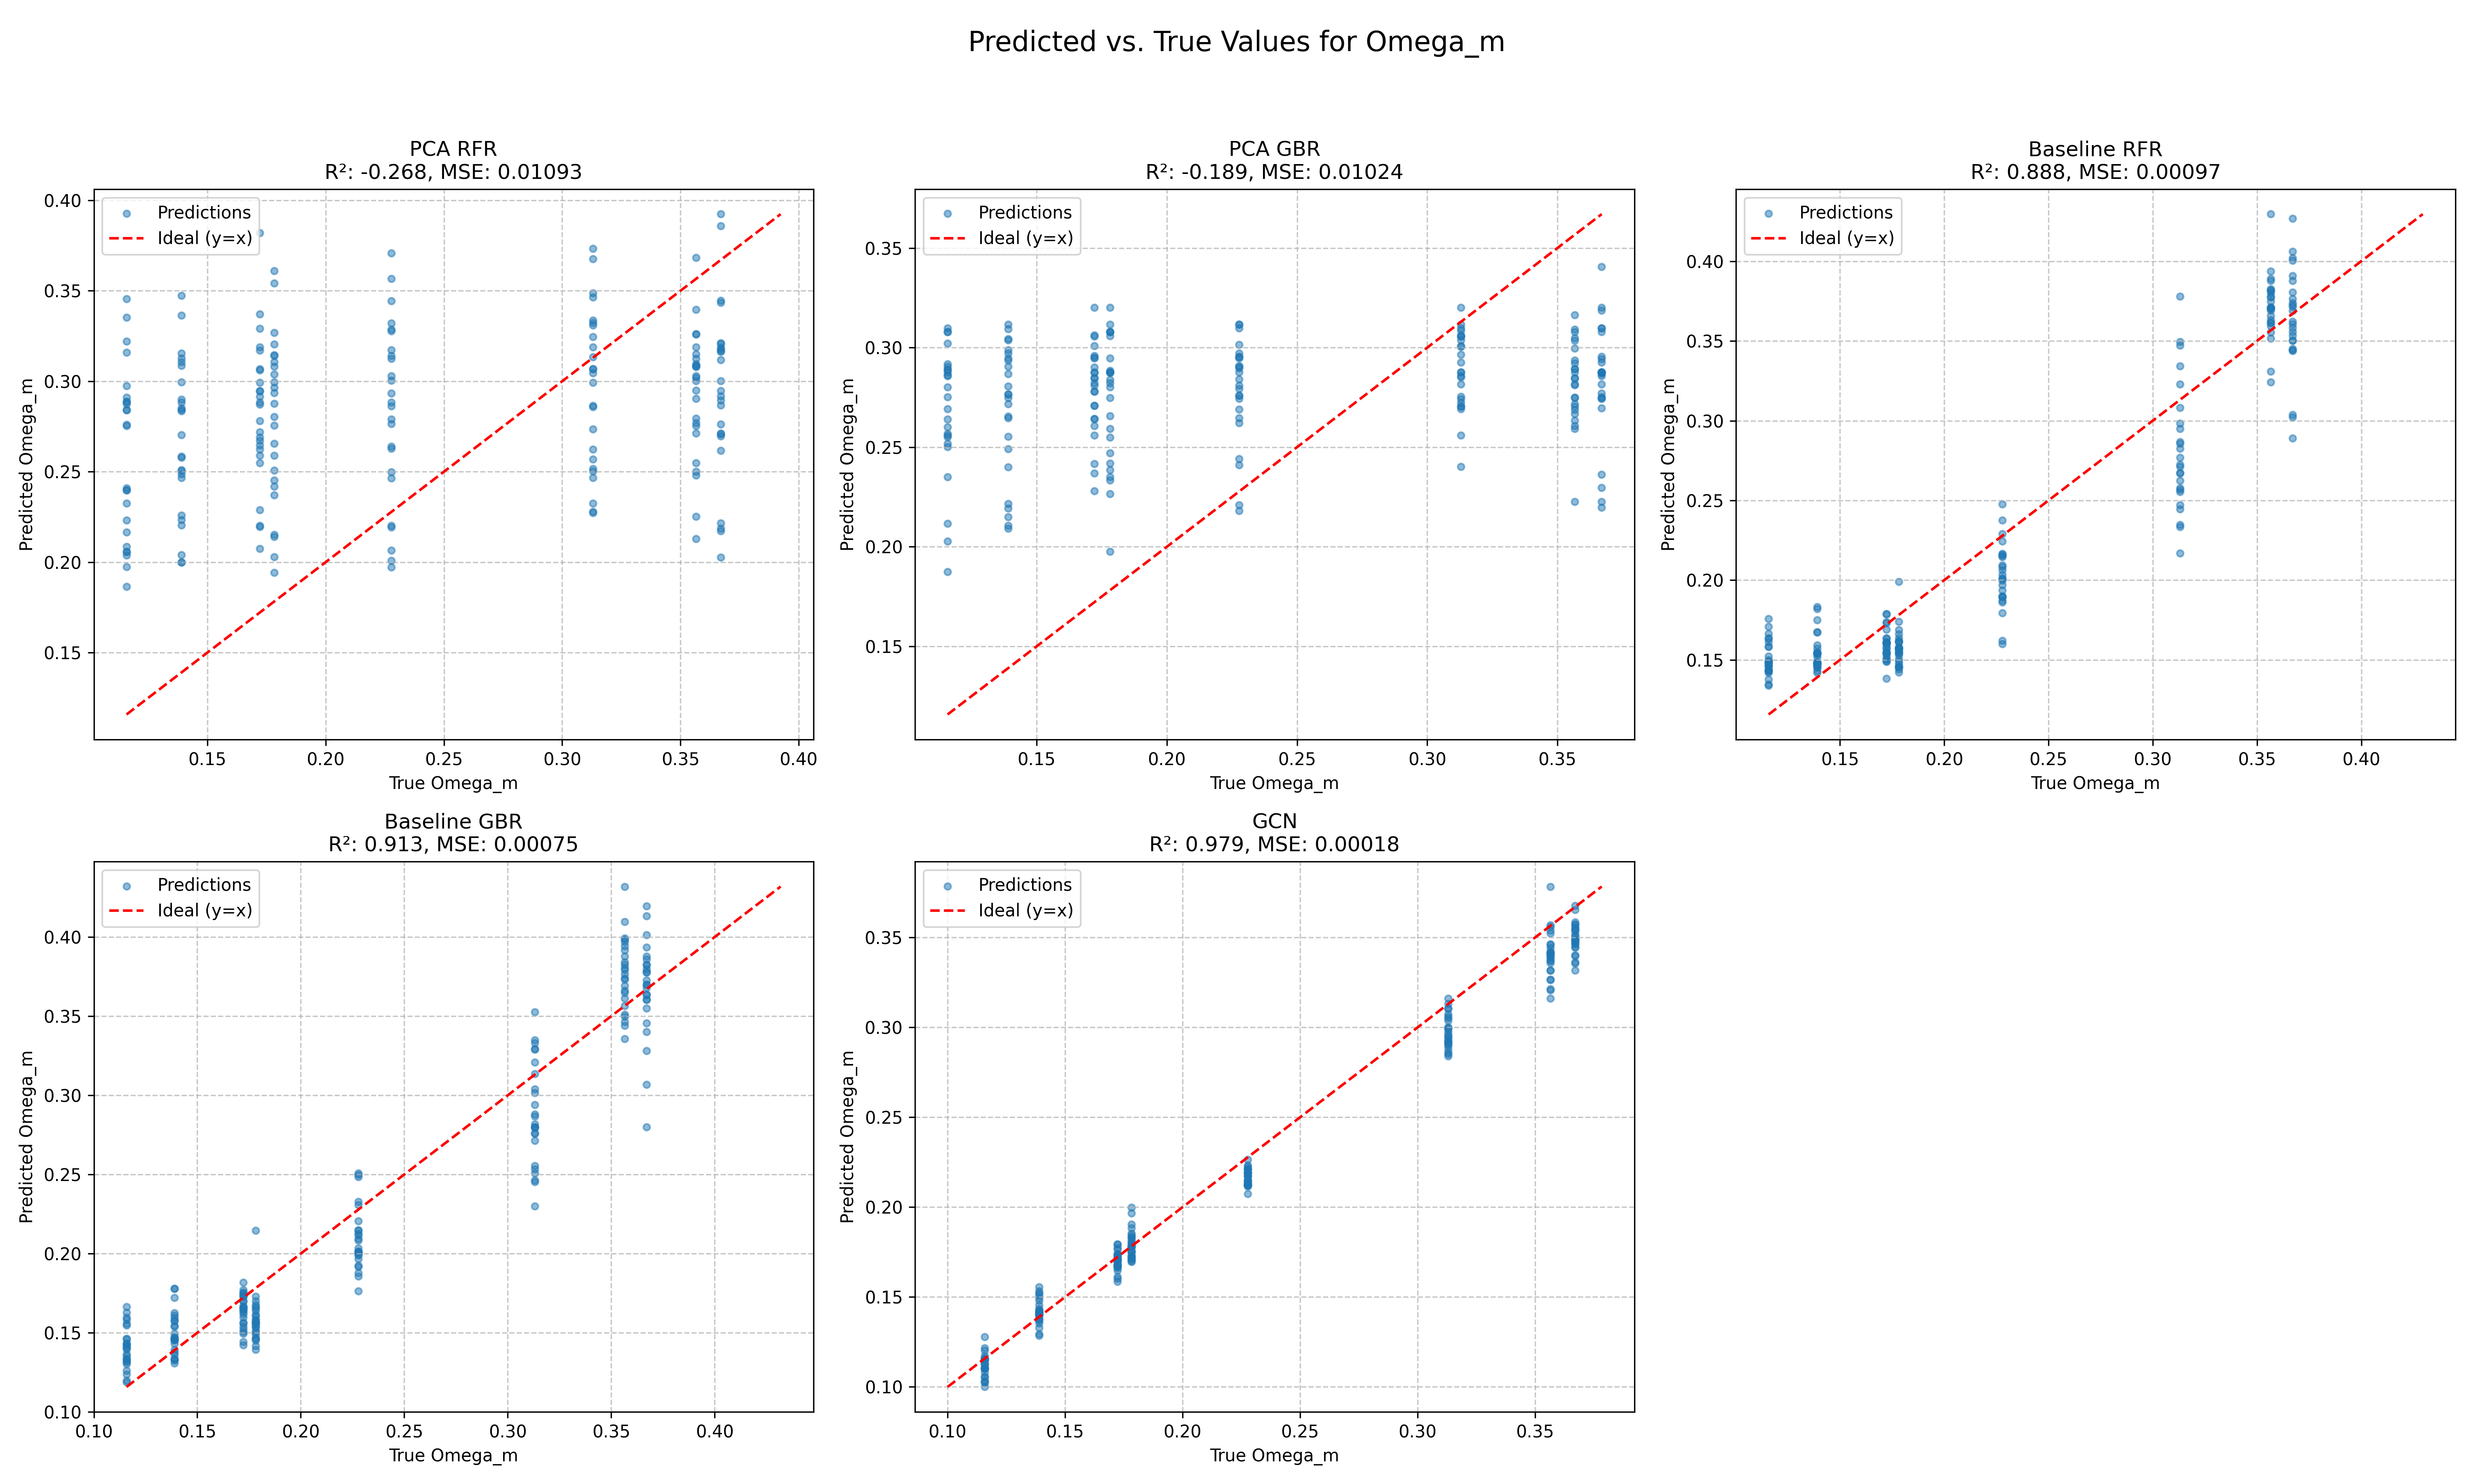
\includegraphics[width=0.5\textwidth]{../input_files/plots/predicted_vs_true_Omega_m_9_20250527-135752.png}
    \caption{Scatter plots of predicted vs. true values of $\Omega_m$ for different models. The GCN and baseline models show a strong positive correlation, while the PCA-engineered feature models show no clear correlation, indicating the superior performance of the former in predicting $\Omega_m$ from merger tree data.}
    \label{fig:predicted_vs_true_omega_m}
\end{figure}

\begin{figure}[h!]
    \centering
    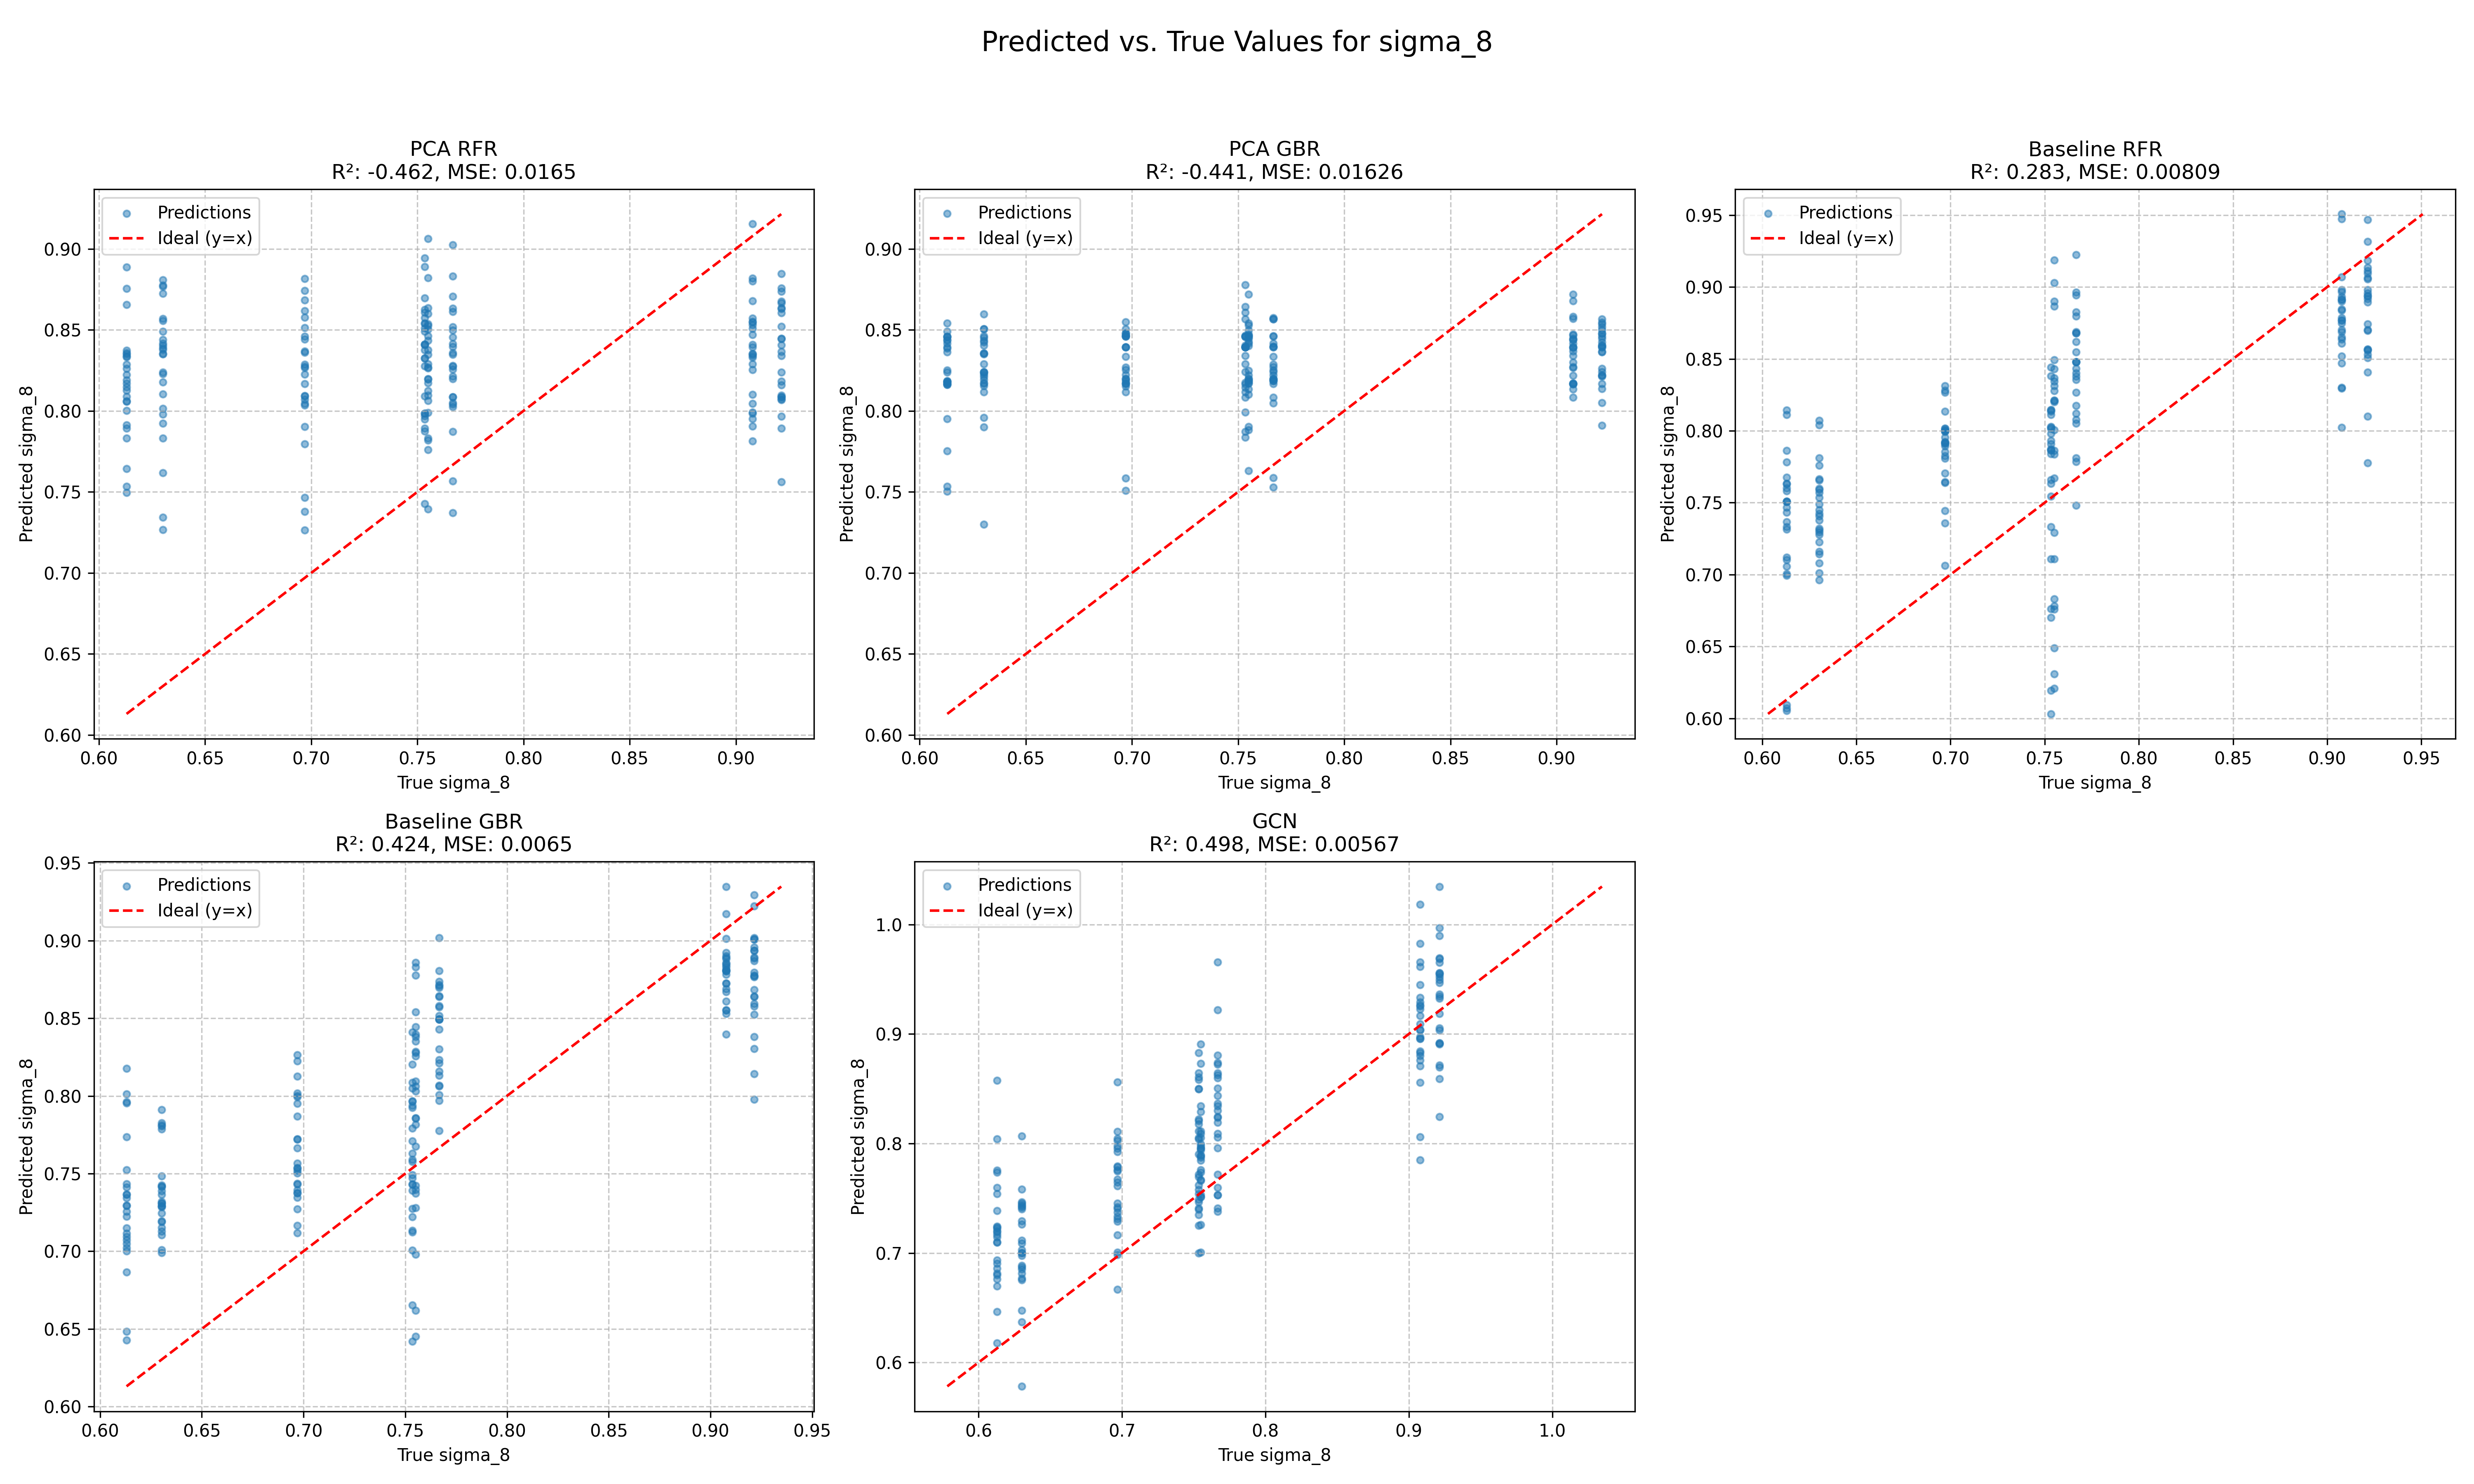
\includegraphics[width=0.5\textwidth]{../input_files/plots/predicted_vs_true_sigma_8_10_20250527-135752.png}
    \caption{Scatter plots of predicted vs. true values for $\sigma_8$ using different feature sets and models: PCA-transformed engineered features with Random Forest Regressor (RFR) and Gradient Boosting Regressor (GBR), baseline aggregated node features with RFR and GBR, and a Graph Convolutional Network (GCN). The GCN and baseline models show positive correlations, whereas the PCA-engineered feature models show little to no correlation, indicating poor predictive performance.}
    \label{fig:predicted_vs_true_sigma_8}
\end{figure}

\subsection{Feature Importance Analysis}

Feature importances were derived for the tree-based models (RFR and GBR). These importances are visualized in the plots `data/feature\_importances\_Omega\_m\_7_<timestamp>.png` and `data/feature\_importances\_sigma\_8\_8_<timestamp>.png`.

\begin{figure}[h!]
    \centering
    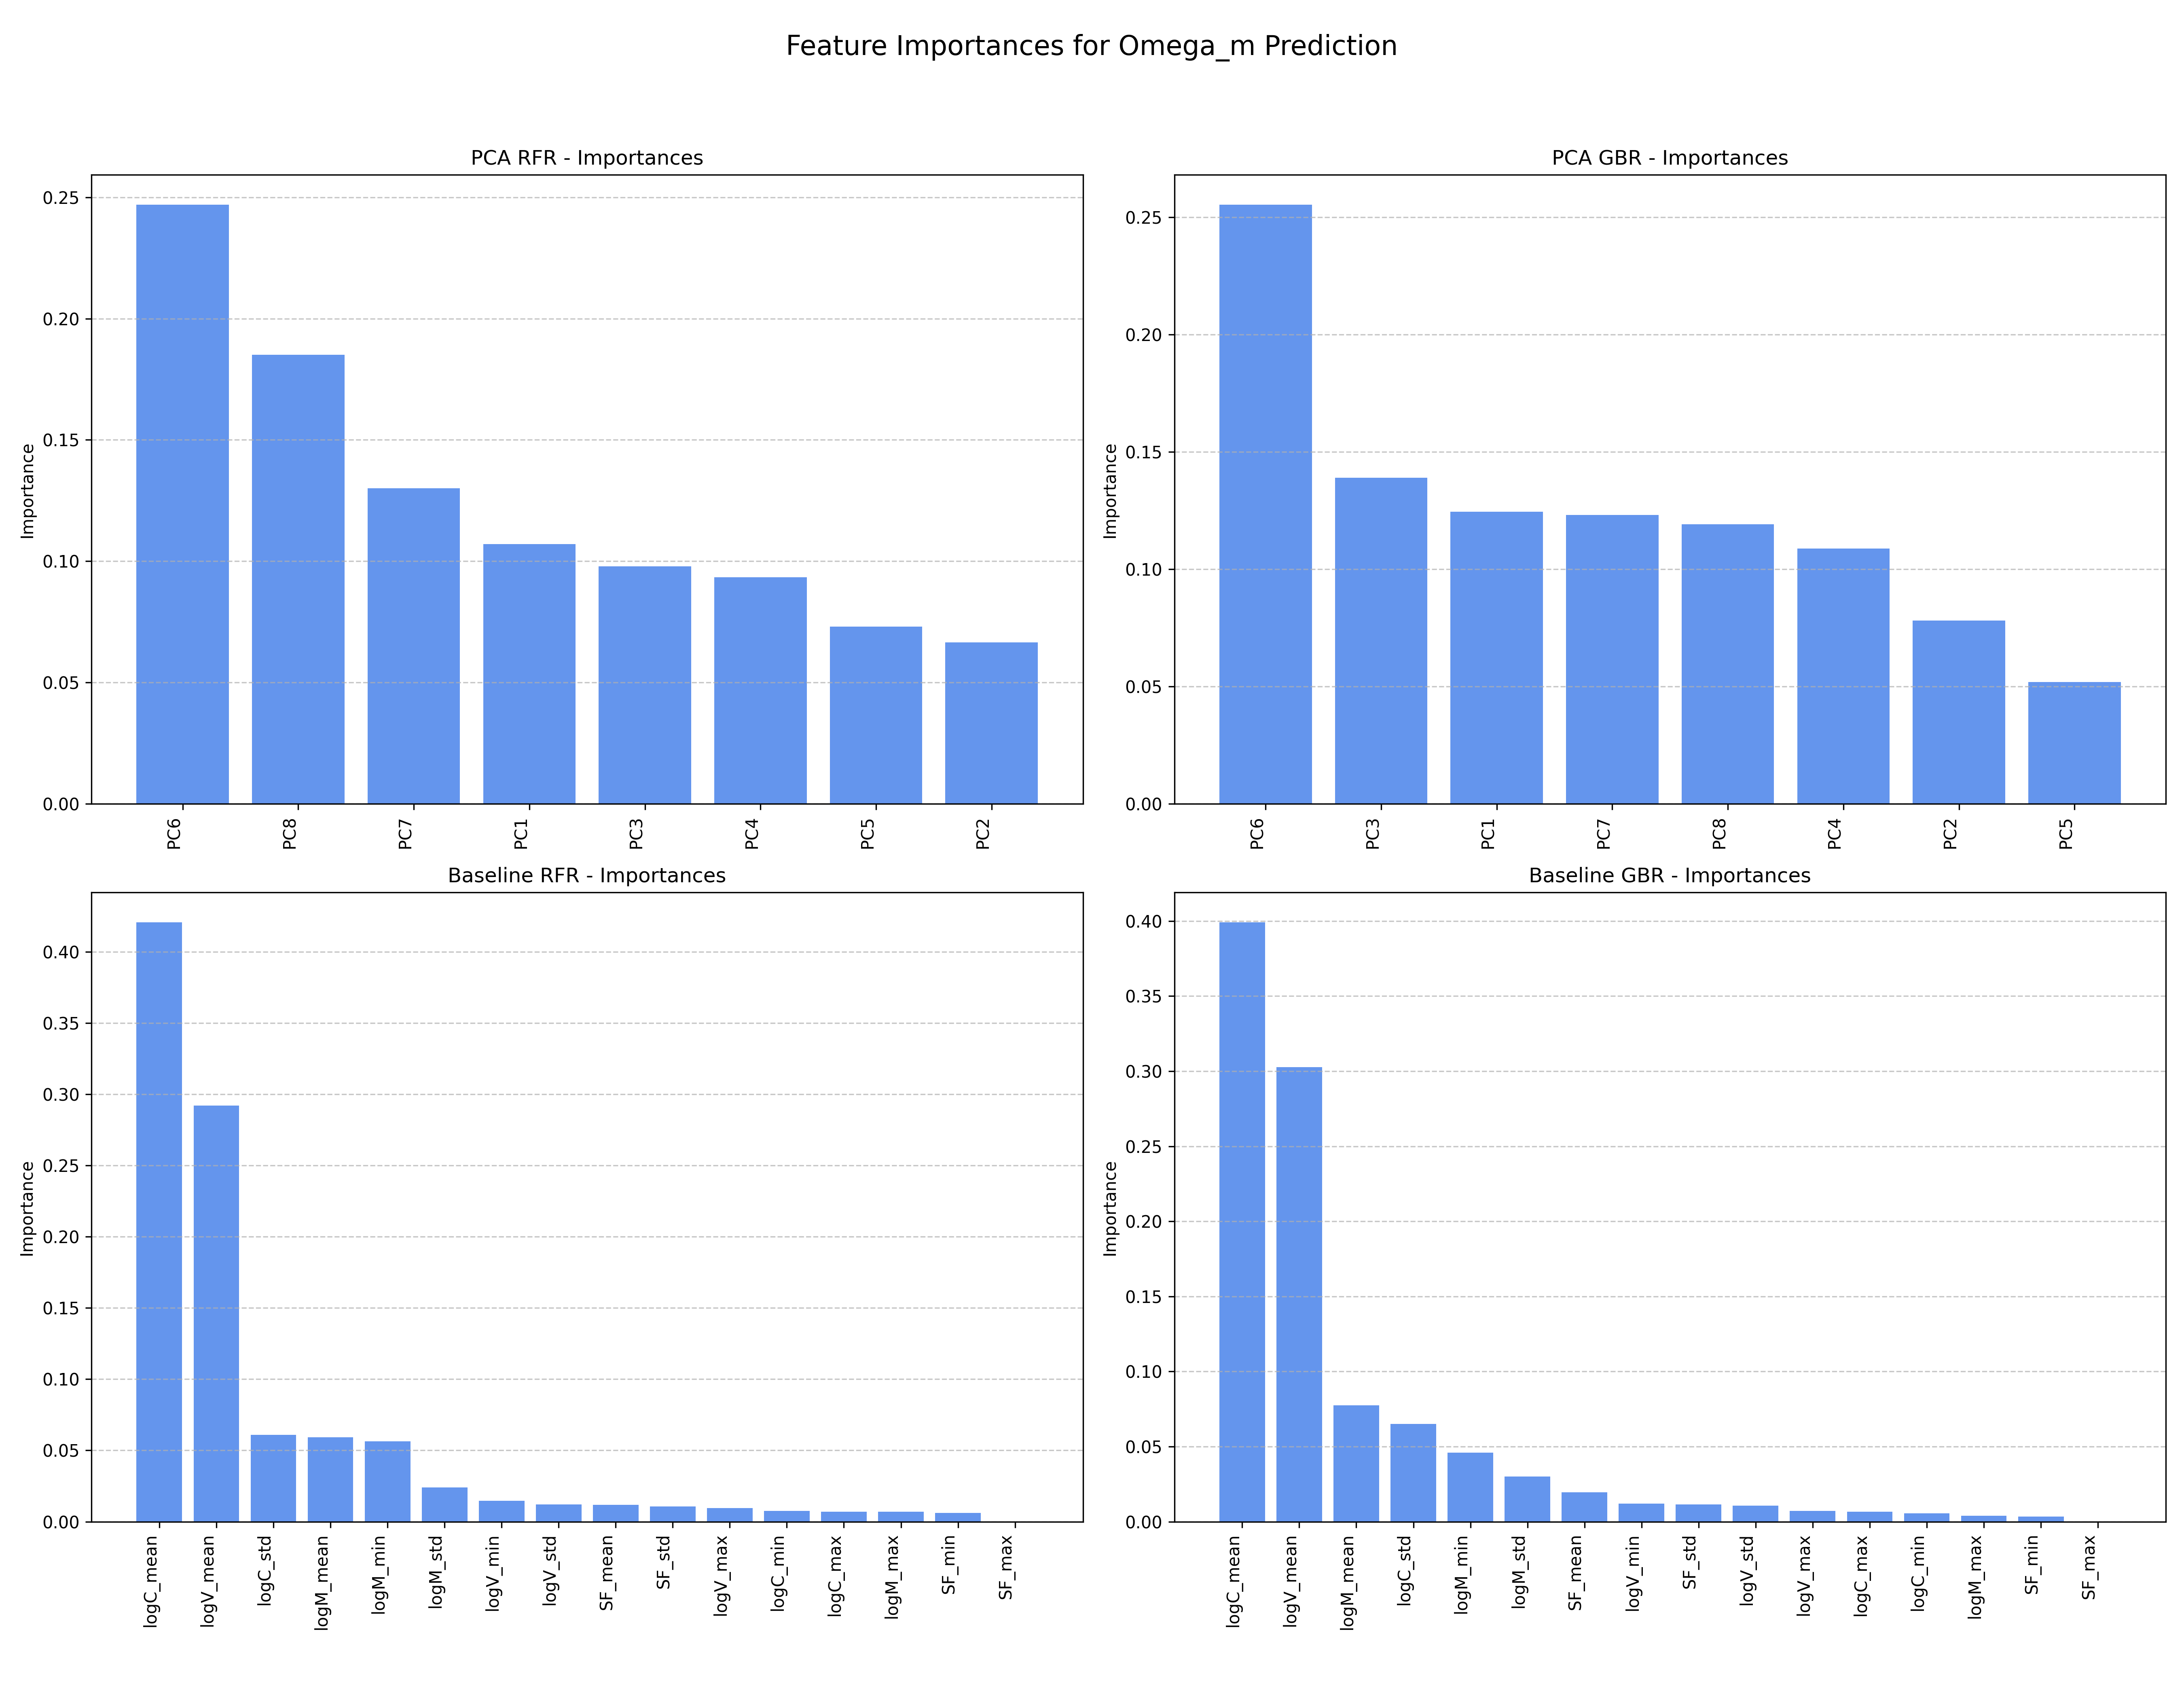
\includegraphics[width=0.5\textwidth]{../input_files/plots/feature_importances_Omega_m_7_20250527-135752.png}
    \caption{Feature importances for predicting $\Omega_m$ using Random Forest Regressor (RFR) and Gradient Boosting Regressor (GBR) models, trained on PCA-transformed engineered features and baseline aggregated node features. The baseline models show that average halo properties such as concentration and Vmax are important predictors, whereas the engineered features show no clear importance.}
    \label{fig:feature_importances_omega_m}
\end{figure}

\begin{figure}[h!]
    \centering
    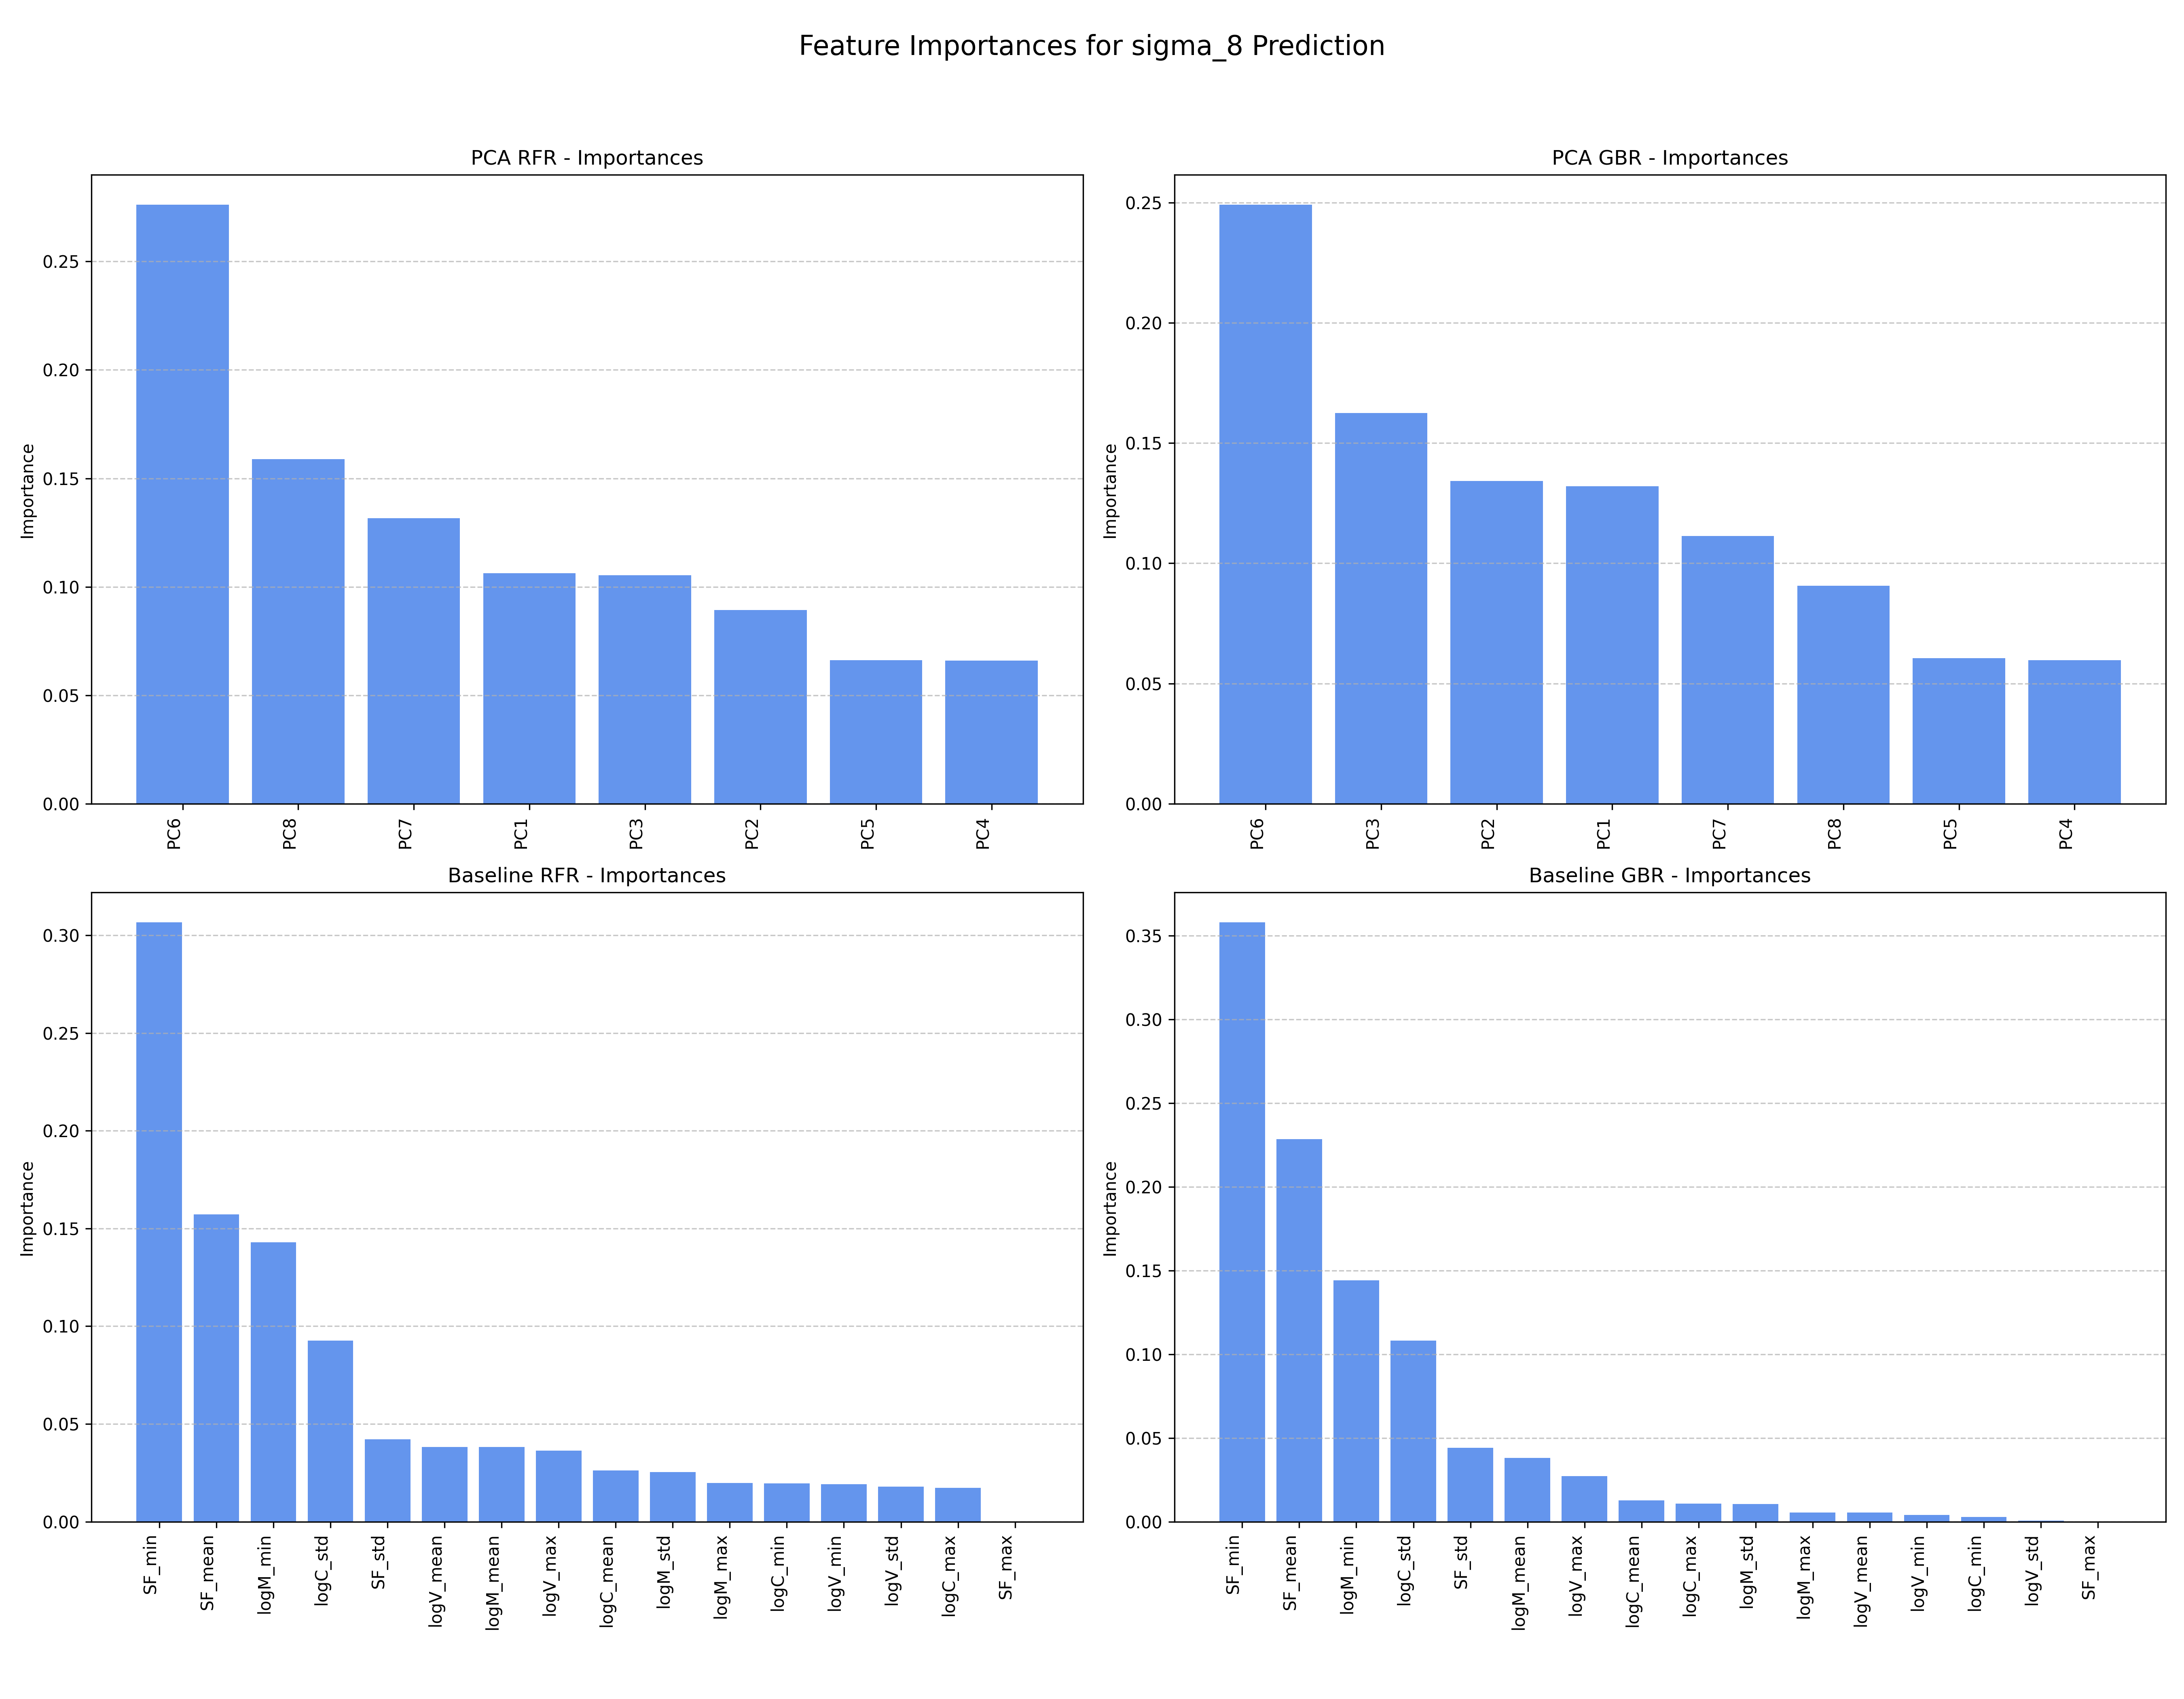
\includegraphics[width=0.5\textwidth]{../input_files/plots/feature_importances_sigma_8_8_20250527-135752.png}
    \caption{Feature importances for predicting $\sigma_8$ using Random Forest Regressor (RFR) and Gradient Boosting Regressor (GBR) models, based on PCA-transformed engineered features and baseline aggregated node features. The baseline models highlight the importance of mean scale factor, mass, and concentration, while PCA-transformed features show varied importances across principal components, but ultimately lead to poor predictive performance.}
    \label{fig:feature_importances_sigma_8}
\end{figure}

\subsubsection{For Baseline Aggregated Node Features}
\begin{itemize}
    \item Predicting $\Omega_m$:
    The RFR model highlighted `SF\ensuremath{\_}mean` (mean scale factor of halos in the tree) as highly important, followed by `logM\ensuremath{\_}mean` (mean log mass) and `logV\ensuremath{\_}mean` (mean log Vmax). The GBR model also emphasized `SF\ensuremath{\_}mean`, `logM\ensuremath{\_}mean`, and `logV\ensuremath{\_}mean`, along with `SF\ensuremath{\_}std` (std of scale factor). This suggests that the average formation time (indicated by scale factor) and average mass/potential well depth of halos in a merger tree are strong indicators of $\Omega_m$.
    \item Predicting $\sigma_8$:
    For RFR, `logM\ensuremath{\_}max` (maximum log mass in the tree), `SF\ensuremath{\_}mean`, and `logC\ensuremath{\_}mean` (mean log concentration) were among the top features. For GBR, `logM\ensuremath{\_}max`, `SF\ensuremath{\_}mean`, and `logM\ensuremath{\_}mean` showed notable importance. The importance of maximum mass and concentration metrics for $\sigma_8$ is plausible, as $\sigma_8$ relates to the amplitude of matter fluctuations, influencing the formation of massive structures and their concentrations.
\end{itemize}

\subsubsection{For Engineered Features + PCA}
The feature importances are for the 8 Principal Components (PC1 to PC8). Predicting $\Omega_m$ and $\sigma_8$: For both targets and both RFR/GBR models, various PCs showed some importance, but no single PC consistently dominated across all models and targets. Interpreting these PC importances directly in terms of the original 24 engineered features is challenging without analyzing the PCA loadings. However, given the overall poor performance of these PCA-reduced features, the specific importances of these PCs are less critical than the observation that they collectively failed to capture predictive signals.

\subsection{Discussion of Engineered Graph Features' Performance}

The most striking outcome of this study is the extremely poor performance of the sophisticated graph spectral and diffusion geometry features, even after PCA. The negative R² values indicate that these features, as implemented and processed, were detrimental to prediction compared to a simple mean prediction. Several factors likely contributed to this:

\subsubsection{Information Loss due to MAX\_NODES\_FOR\_EIGS and Imputation}
A large fraction of graphs (638/800 training, 164/200 testing) had their spectral and diffusion features replaced by NaNs because they exceeded the 500-node limit for eigenvalue computation. These NaNs were then mean-imputed. This imputation strategy, applied to a majority of the data for these 20 features, likely homogenized the feature values, masked true structural variations, and introduced noise, severely degrading their informational content. The distributions plotted in `engineered\_feature\_dist\_laplacian\_*.png` and `engineered\_feature\_dist\_diff\_*.png` are likely dominated by these imputed means for many graphs.

\subsubsection{Insensitivity of Chosen Features or Aggregation}
The specific spectral moments (mean, std, skewness, kurtosis of eigenvalues, sum of smallest eigenvalues) and the aggregation of diffusion map eigenvectors (mean, max, min pooling) might not be the most sensitive probes of cosmological information encoded in merger tree morphology. These global summaries might average out subtle but crucial structural differences.

\subsubsection{Suboptimal PCA Transformation}
While PCA reduces dimensionality by maximizing variance, it is an unsupervised method. The components that explain most of the variance in the feature space are not necessarily the most predictive for the cosmological parameters. It's possible that information relevant to $\Omega_m$ and $\sigma_8$ was present in lower-variance components that were discarded, or that the linear transformation of PCA was insufficient to disentangle complex relationships.

\subsubsection{Coarseness of Edge Features}
The mean and variance of scale factor differences and log mass ratios might be too simplistic to capture the nuances of merger histories.

\subsubsection{Intrinsic Difficulty}
The relationship between these specific graph-theoretic properties and cosmology might be inherently weak or highly non-linear, making it difficult for traditional regressors to capture, even with perfect features.

The failure of these "classical" geometric deep learning inspired features underscores the challenge in manual feature engineering for complex graph data, especially when computational constraints lead to compromises in feature calculation.

\subsection{Comparison with Baseline Approaches and Physical Implications}

The Baseline Aggregated Node Features significantly outperformed the engineered features. For $\Omega_m$, R² values reached up to 0.9134 (GBR), and for $\sigma_8$, up to 0.4238 (GBR). This implies that simple global statistics of halo properties (average mass, concentration, Vmax, and particularly average scale factor, as indicated by feature importances) within a merger tree are strongly correlated with $\Omega_m$ and moderately correlated with $\sigma_8$. Physically, this suggests that cosmologies with different $\Omega_m$ values produce merger trees with distinguishably different average halo properties and formation epochs. For instance, a higher $\Omega_m$ might lead to earlier formation and thus lower average scale factors in trees, which was picked up by the `SF\ensuremath{\_}mean` feature.

The GCN model demonstrated the best performance overall, achieving an R² of 0.9786 for $\Omega_m$ and 0.4977 for $\sigma_8$. This highlights the strength of GNNs in learning relevant representations directly from raw node features and graph connectivity. GCNs can automatically discover complex, non-linear patterns and feature interactions that are difficult to hand-engineer. The GCN's success, particularly its improvement over the strong baseline, suggests that not only the global average of node properties but also their specific arrangement and relationships within the tree structure (i.e., the graph topology itself) carry cosmological information. The GCN effectively learns a "graph embedding" that is optimized for the prediction task.

The significantly better performance for $\Omega_m$ compared to $\sigma_8$ across all successful methods (Baseline and GCN) suggests that merger tree morphology, as characterized by the input node features, is more sensitive to changes in the matter density parameter than to the amplitude of matter fluctuations on 8 $h^{-1}$Mpc scales.

\subsection{Summary}

In summary, the sophisticated graph spectral and diffusion geometry features performed poorly, likely due to computational limitations and subsequent imputation. Simpler aggregated node features showed significant predictive power, especially for $\Omega_m$, suggesting a strong connection between average halo properties and the matter density parameter. The GCN model achieved the best overall performance, demonstrating the potential of graph neural networks to automatically learn cosmologically relevant information directly from merger tree structures. The GCN's superior performance, particularly for $\Omega_m$, underscores the importance of considering not only global halo properties but also the specific arrangement and relationships within the merger tree structure.

\end{document}
                